% interactcsesample.tex
% v1.05 - August 2017

\documentclass[]{interact}

\usepackage{epstopdf}% To incorporate .eps illustrations using PDFLaTeX, etc.
\usepackage[caption=false]{subfig}% Support for small, `sub' figures and tables
\usepackage{color}


\usepackage{natbib}% Citation support using natbib.sty

\theoremstyle{plain}% Theorem-like structures provided by amsthm.sty
\newtheorem{theorem}{Theorem}[section]
\newtheorem{lemma}[theorem]{Lemma}
\newtheorem{corollary}[theorem]{Corollary}
\newtheorem{proposition}[theorem]{Proposition}
\theoremstyle{definition}
\newtheorem{definition}[theorem]{Definition}
\newtheorem{example}[theorem]{Example}
\theoremstyle{remark}
\newtheorem{remark}{Remark}
\newtheorem{notation}{Notation}


\usepackage{amsmath}
\usepackage{amsthm,amsfonts}
\usepackage{graphicx}
\usepackage{bm}
\usepackage{xparse}
\usepackage[utf8]{inputenc}
\usepackage{mathrsfs}
\usepackage{bbm}

\def\Expect{{\mathbb E}}
\def\Prob{{\mathbb P}}
\def\minimize{\mathop{\rm minimize}}
\def\maximize{\mathop{\rm maximize}}
\def\subto{{\rm subject \mbox{   }\rm to}}
\def\min{\mathop{\rm min}}
\def\max{\mathop{\rm max}}
\def\argmax{\mathop{\rm argmax}}
\def\argmin{\mathop{\rm argmin}}
\def\sup{\mathop{\rm sup}}
\def\inf{\mathop{\rm inf}}
\newcommand{\ie}{{\it i.e., }}
\newcommand{\eg}{\textit{e.g.}}
\newcommand{\V}[1]{{{\boldsymbol #1}}}
\renewcommand{\x}{\V{x}}
\newcommand{\X}{\mathcal{X}}
\newcommand{\e}{\V{e}}
\newcommand{\0}{\V{0}}
\newcommand{\1}{\V{1}}
\newcommand{\Dist}{\mathcal{D}}
\newcommand{\mymbox}[1]{\mbox{\scriptsize #1}}
\renewcommand{\Re}{\mathbb{R}}
\newcommand{\quoteIt}[1]{``#1''}
\newcommand{\support}[1]{\1_{[#1]}}
\newcommand{\Halmos}{{\qed}}
\newcommand{\eye}{{I}} %I matrix

\newcommand{\EDmodified}[1]{{\color{red} #1}}
\newcommand{\EDcomments}[1]{{\EDmodified{Erick commented: #1}}}
%\newcommand{\EDcomments}[1]{{}}
\newcommand{\modified}[1]{{\color{blue} #1}}
\newcommand{\removed}[1]{{}}

\def\epi{\mathop{\rm epi}}
\def\diag{\mathop{\rm epi}}
\def\dom{\mathop{\rm dom}}
\def\tr{\mathop{\rm tr}}
\def\Var{\mathop{\rm Var}}
\def\CE{\mathop{\rm CE}}
\def\Cov{\mathop{\rm CE}}
\def\sign{\mathop{\rm sign}}
\def\EU{\mathop{\rm EU}}

\newcommand{\iso}{\simeq}
\newcommand{\dd}{\partial}
\newcommand{\normal}{\mathscr{N}}
\newcommand{\trueRisk}{R_{\mathrm{true}}}
\newcommand{\uInv}{u^{-1}}
\newcommand{\qHat}{{\hat q}}
\newcommand{\qStar}{{q^\star}}
\newcommand{\xMax}{\xi}
\newcommand{\grad}{\nabla}







\theoremstyle{plain}
\newtheorem{prop}{Proposition}
\newtheorem{thm}{Theorem}
\newtheorem{coro}{Corollary}
\newtheorem*{thm*}{Theorem}
\newtheorem{claim}{Claim}
\newtheorem{assumption}{Assumption}
\theoremstyle{definition}
\newtheorem*{rem}{Remark}
\newtheorem*{ex}{Example}


\title{Generalization Bounds for Regularized Portfolio Selection with Market Side Information}

\author{
\name{Thierry Bazier-Matte\textsuperscript{a} and Erick Delage\textsuperscript{b}\thanks{CONTACT T. Bazier-Matte at \texttt{tbaziermatte@cdpq.ca} and E. Delage at \texttt{erick.delage@hec.ca}. E. Delage gratefully acknowledges the support of the
    Canadian Natural Sciences and Engineering Research Council [RGPIN-2016-05208].}}
\affil{\textsuperscript{a}Caisse de dépôt et placement du Québec, Canada.}
\affil{\textsuperscript{b}HEC Montreal, Canada.}
}

\begin{document}
\maketitle

\begin{abstract}
%  In recent years,  much pressure has been applied in order to allow portfolio management theory to address was required to evolve in order to  
  Drawing on statistical learning theory, we derive out-of-sample and optimality
  guarantees about the investment strategy obtained from a regularized portfolio
  optimization model which attempts to exploit side information about the financial market
  in order to reach an optimal risk-return tradeoff. This side information might include
  for instance recent stock returns, volatility indexes, financial news indicators,
  etc. In particular, we demonstrate that a regularized investment policy that linearly combines this
  side information in a way that is optimal from the perspective of a random sample set is
  guaranteed to perform also relatively well (\ie, within a perturbing factor of
  $O(1/\sqrt{n})$) with respect to the unknown distribution that generated this sample
  set.    We also demonstrate that these performance guarantee are lost in a high-dimensional regime
  where the size of the side information vector is of an order that is comparable to the
  sample size.  We further extend these results to the case where non-linear investment policies are considered using a kernel operator and show that with radial basis function kernels the performance guarantees become insensitive to how much side information is used. Finally, we illustrate our findings with a set of numerical experiments involving financial data for the NASDAQ composite index.

  % \Erick{Voici l'ancien abstract: Drawing on statistical learning theory, we propose a
  %   robust portfolio optimization mechanism agnostic to market distribution based on side
  %   information and on market returns. In particular, we exhibit a linear investment
  %   policy based on the risk preferences of an investor and on a sample of the market and
  %   show that out-of-sample and suboptimality guarantees on the quality of the certainty
  %   equivalent of the proposed investment can be provided. In addition, we also consider
  %   the high-dimensional case where the number of these side informations is of the order
  %   of the sample size. }
\end{abstract}

\begin{keywords}
Portfolio optimization; Generalization bound; Utility maximization; learning theory
\end{keywords}

%\input{intro}
\section{Introduction}
\label{sec:intro}

There is no doubt that modern portfolio management theory has been dramatically affected
by two important historical events. First, Markowitz in 1952 highlighted in his seminal
paper \cite{markowitz1952portfolio} how investment decisions needed to inherently
trade-off between risk (typically measured using variance) and returns (in the form of
expected returns). This was later reinterpreted as a special case of characterizing risk
aversion using expected utility theory \cite{neumann44:tgeb}.  The flexibility of such a
theory has since then been demonstrated in many occasions regarding the wide diversity of
investors' risk aversion that it can represent (see \cite{ingersoll87} and reference
therein for an overview of the type of attitudes that can be modeled).

The second turning point of this theory can be considered to have occurred with the
financial crisis of 2008 which provided strong evidence that the use of statistics such as
variance and value-at-risk, and of distribution models that are calibrated using historical data could
provide a false sense of security \cite{Salmon09}.  In an attempt to address some of these
new challenges, researchers have proposed using more robust statistical estimators (see
\cite{madan1998variance,goldfarb03,olivares2015robust}) while others encouraged the use of
robust portfolio management models that are designed to produce out-of-samples guarantees
by exploiting the use of a confidence region for the distribution of future returns
(See \cite{delageYe10,huangzhu10,Esfahani15,VanPary2017}).
%Delage and Ye, 

In this work, we draw on statistical learning theory to establish what are the
out-of-sample guarantees that can be obtained when using regularization in an expected
utility model that allows to exploit side information about the financial markets (see
\cite{brandt2009parametric} where a non-regularized version of this model was introduced).  This side
information could consist of fundamental analysis (as was famously done in
\cite{fama1993common}), but also of technical analysis, financial news, etc. Overall,
we consider our contribution to be four-fold.
\begin{enumerate}
\item\label{contrib:1} We derive a lower bound on the out-of-sample performance of the investment strategy
  returned by this regularized model.  In this respect, our results differ from the usual
  statistical learning and stability theory results in the sense that our guarantees will
  not be in terms of quality of fit of a model (\eg, expected squared loss, hinge loss,
  etc.), but rather in terms of the actual performance perceived by the investor (through
  the notion of a certainty equivalent).
\item\label{contrib:2} We derive an upper bound on the suboptimality of the investment strategy when
  compared to the optimal strategy that would be derived using the full knowledge of the
  sample distribution. Note that, \modified{to the best of our knowledge}, such finite sample guarantees have not yet been established for distributionally robust optimization models.
\item\label{contrib:3} Considering that nowadays a growing amount of side-information can be exploited by
  individuals to make their investments, we establish precisely how these bounds are
  affected at a high-dimensional (or ``big data'') regime.
  \item\label{contrib:4} Finally, we present how the out-of-sample and sub-optimality bounds can be extended to a multi-asset portfolio selection problem and a ``kernelized'' single-asset portfolio selection problem which can produce investment strategies that are linear functions of a lifting of the side-information to a possibly infinite dimensional space.
\end{enumerate}
It is worth mentioning that contributions \ref{contrib:1} - \ref{contrib:3} are similar in spirit to those of \cite{rudin2015big} who applied stability theory to provide generalization bounds for a newsvendor problem. There are however a number of distinctions regarding how stability theory needs to be articulated for the two applications. For example, our paper deals with a more general performance function which is non-linear and possibly unbounded on both sides, and needs to identify reasonable assumptions about the financial market in order for an optimal investment strategy to exist. 
%we focus on generalization and sub-optimality bounds which, in our opinion, are more informative than the measure that is bounded in \cite{rudin2015big}. Moreover, we attempt to be more precise in our analysis on characterizing the effect of data dimensionality on the out-of-sample performance.
%\footnote{Relevant historical facts for reviewer's eye only: Throughout the different versions of \cite{rudin2015big}, the authors have made confusing statements about how regularization allows one to control the effect of data dimensionality on out-of-sample performance guarantees. See for instance in Theorem 6 of the version revised in Nov 2017 where a typo in the reporting of the bound let's an inattentive reader conclude that the bound is not sensitive to $p$ which was previously an important message of this section.} 
To the best of our knowledge, Contribution \ref{contrib:4} is also entirely original (and could be of use to the newsvendor problem) given that the work of \cite{rudin2015big} did not consider a multi-dimensional decision vector and that it used kernels in the context of kernel density estimator unlike in this work where a kernel operator will be used to define the space of possible investment strategies. 

In the field of finance, it is worth mentioning that \cite{GOTOH2012371} did employ machine learning theory to establish out-of-sample performance guarantees of portfolios, yet they solely focus on the out-of-sample probability of reaching a target return (a.k.a. loss probability minimization), instead of a more general expected utility model, and did not consider the use of market side information. The learning algorithm that is proposed by the authors is also very different in spirit to ours as it suggests minimizing a ratio between value-at-risk (or regularized conditional value-at-risk) and the norm of the portfolio for different confidence level instead of simply minimizing a regularized version of the performance measure of interest, as would be done in our approach. Finally, the authors do not provide an out-of-sample guarantee on suboptimality of the optimal in-sample portfolio and perhaps more importantly do not  establish whether the out-of-sample performance of the in-sample optimal portfolio converges to the best possible out-of-sample performance as more observations are made. One can also identify some interesting applications of kernels (e.g. in \cite{Gyorfi06nonparametrickernel-based} and \cite{TAKANO20143901}) to dynamic portfolio selection but none of this prior work studies the out-of-sample performance in one shot investment problem where side-information can be exploited. 

The rest of the paper is divided as follows. First, we formally introduce our model and
assumptions in Section \ref{sec:model}. Section \ref{sec:oos} then presents what kind of
out-of-sample guarantees can be provided on the certainty equivalent (CE) of the investor
using a sample of market returns and side information when assuming a stationary market
distribution. We then proceed in Section \ref{sec:sub} to show that the same kind of
guarantees can also be derived for the CE suboptimality, before showing in Section
\ref{sec:bigdata} what kind of behaviour can be expected in ``big-data'' situation. We
then present extensions of our results to the case of multiple risky assets in Section \ref{sec:multiassets} and to the case where investment strategies are defined using kernels in Section \ref{sec:kernel}. Finally, in Section \ref{sec:num} we illustrate our findings in a set of numerical experiments and conclude in Section \ref{sec:conc}. All proofs have been pushed to the appendix. %Additional discussions on this topic can also be found in \cite{ThierryThesis}, i.e., the thesis from which these results are drawn. 




%\input{model}
\section{Model and Assumptions}\label{sec:model}
% \newcommand{\Expect}{E}
\newcommand{\F}{F}
\newcommand{\Fhat}{{\hat{\F}}}
\newcommand{\qhat}{{\hat{q}}}
\newcommand{\Sx}{{\mathcal{S}_X}}
\newcommand{\Sr}{{\mathcal{S}_R}}
\newcommand{\Sn}{\mathcal{S}_n}
\newcommand{\urange}{u_{\mbox{\footnotesize range}}}
%\newcommand{\umin}{u_{\mbox{\footnotesize min}}}
%\newcommand{\qhatOp}{{\bold{\qhat}}}
\newcommand{\investA}{{\pi}}





%\newcommand{\EUFq}{\mbox{EU($q;\F$)}}
%\newcommand{\EUFhqh}{\mbox{EU($\qhat;\Fhat$)}}
%\newcommand{\EUFqh}{\mbox{EU($\qhat;\F$)}}
%\newcommand{\CEFq}{\mbox{CE($q;\F$)}}
%\newcommand{\CEFhqh}{\mbox{CE($\qhat;\Fhat$)}}
%\newcommand{\CEFqh}{\mbox{CE($\qhat;\F$)}}





We consider a classical financial portfolio selection problem involving a risky asset with
random return rate $R$ and a risk-free asset with return rate of $0\%$ for simplicity of exposure. We
also suppose that the investor's risk aversion can be characterized using expected utility
theory using a strictly increasing concave utility function $u$, and that the investor has
access to side information regarding the returns. This information might be the result of
processing the most recent financial or economic news, etc. We let this information be
described as a vector of $p$ normalized random features $X\in\Re^p$. In this
context, if the the distribution $\F$ of the pair $(X,R)$ of side information and return
is known, a linear investment policy that exploits the side information optimally for this
investor can be obtained by solving the following optimization problem:
\begin{equation}
\maximize_{q\in\Re^p}\;\;\;\Expect_\F[u(R\cdot q^TX)]\;,\label{EUF}
\end{equation}
\modified{where an investment policy consists of investing a $q^T X$ proportion of the wealth in the risky asset and a $1-q^T X$ proportion in the risk-free one,} and where it is assumed that short-selling is permitted.\footnote{\modified{Note that in the case that the risk free return rate is non-null, one should interpret $R$ as the return in excess of the risk-free rate. Hence, the model can still take the form presented in \eqref{EUF} using the reduction $\Expect_\F[u((R+r_f)\cdot q^T X + r_f(1-q^T X))]=\Expect_\F[u(R\cdot q^T X + r_f)]=\Expect_\F[v(R\cdot q^T x)]$ where $v(y):=u(y + r_f)$.} }

In practice however, the exact distribution describing the relation between $X$ and $R$ is
not available at the time of designing the investment policy and one might instead need to
exploit a sample set $\Sn:=\{(x_i,r_i)\}_{i=1}^n$ were each $(x_i,r_i)$ was drawn independently and identically from
$\F$. Unfortunately, when the sample size $n$ is relatively small compared to $p$, it is
well known that the version of problem \eqref{EUF} that uses the empirical distribution $\Fhat$ obtained
from sample $\Sn$ can suffer from overfitting the sample and produce investment policies that
perform badly out of sample. This is for instance illustrated in the following example.

\begin{ex}
  Consider a case where $n=p$ and each term in $X$ is \modified{independently} and
  identically drawn from a Gaussian distribution. Given that it is well known that the
  probability that the random matrix \modified{$\Xi := [X_1\;X_2\;\dots\;X_n]^T$} be singular is null,
  then one can easily establish that problem \eqref{EUF} with $\Fhat$ is
  unbounded. Indeed, one can verify that $r_i \bar{q}^T x_i = 1$ for all $i=1,\dots,n$
  when $\bar{q}$ is set to \modified{${\Xi^{-1}}[1/r_1\;1/r_2\;\dots\;1/r_n]^T$}. Hence, one can
  achieve an arbitrarily large empirical expected utility by investing according to
  $\alpha\bar{q}$ for $\alpha>0$. Note that it would be surprising that such an extreme policy would perform well out-of-sample.
\end{ex}

To prevent issues associated to overfitting, one might instead seek the optimal solution
of the following regularized empirical expected utility maximization problem:
\begin{equation}
\maximize_{q\in\Re^p}\;\;\;\Expect_\Fhat[u(R\cdot q^TX)]-\lambda\|q\|_2^2\;.\label{EUFhatReg}
\end{equation}
We will refer to the optimal solution of this problem as $\qhat$. \modified{Note that such an optimal solution always exists since the objective function is strongly concave.}

The question remains of understanding what guarantees \modified{one has} regarding out-of-sample performance of the portfolio investment policy obtained from such a regularized
problem. In what follows, we establish some high confidence bounds on the out-of-sample performance and suboptimality of $\qhat$.

%\input{oos_performance}
\section{Out-of-sample performance bounds}\label{sec:oos}

In this section, we identify a high confidence bound on the out-of-sample performance of $\qhat$. In particular, since utility functions are expressed in units without any
physical meaning for the investor, any guarantees derived using learning theory should be
reinterpreted in terms of a guarantee on the certainty equivalent\footnote{The fact that
  $c$ is the certainty equivalent of a random return $R$ implies that the  \modified{investor is}
  indifferent between being exposed to the risk of $R$ or getting involved in a risk free
  investment that has a return rate of $c$.} (in percent of return) of the risky
investment produced by $\qhat^T X$. In other words, we will be interested in bounding how
different the in-sample certainty equivalent performance of $\qhat$ might be compared to
the out-of-sample certainty equivalent performance. % Likewise, we will also show how we can
% expect the policy $\hat q$ to converge toward an unknown market optimal investment policy
% based on $u$ and $\lambda$.

In order to shed some light on this question, we first make the following assumptions.

\begin{assumption}\label{ass:R}
\modified{  The random return $R$ is supported on a bounded interval
  $\Sr\subseteq [-\bar{r},\bar{r}]$, for some $\bar{r}\in\Re$, such that $\Prob_F(|R|\leq \bar{r})=1$.}
\end{assumption}

\begin{assumption}\label{ass:X}
\modified{  The random vector of side-information $X$ is supported on a bounded set $\Sx$ such that
  $\Prob_F(\|X\|_2\leq \xi)=1$ for some $\xi\in\Re$.}
\end{assumption}

\begin{assumption}\label{ass:u}
  The utility function is normalized such that $u(0)=0$ and $\lim_{r\to0^+}u'(r) =
  1$. Furthermore, it is Lipschitz continuous with a Lipschitz constant of $\gamma$, i.e.,
  for any $r_1\in\Re$ and $r_2\in\Re$, we have that
  $|u(r_1) - u(r_2)| \leq \gamma|r_1-r_2|$.
\end{assumption}

The first assumption is relatively realistic given that one can usually assess from
historical data a large enough interval of returns which could be assumed to contain $R$
with probability one. For instance, when looking at the last 35 years of daily returns for
an index such as S\&P 500, this interval can legitimately be set to $[-25\% , 25\%]$ daily
returns. If some side information are not known to be bounded, the second assumption might
require one to pre-process the vector of side information in order to rely on the results
that will be presented. This could typically be done by employing a \quoteIt{clipping} procedure that projects this vector on the
surface of a ball of radius $\xi$ when $\|X\|_2>\xi$, which is as simple as replacing $X$
with $(\xi/\|X\|_2)\cdot X$. This assumption will be further studied in Section
\ref{sec:bigdata}. Finally, while the last assumption is fairly common for establishing
generalization bounds and can certainly accommodate any piecewise linear utility function
(often used by numerical optimization methods), it is important to mention that it is not
one that is commonly made in modern portfolio theory. If, for instance, an investor
expresses an absolute risk aversion uniformly equal to $\alpha$, this suggests the use of
$u(r):=(1/\alpha)(1-\exp(-\alpha r))$ which is not Lipschitz continuous. Fortunately, the
theory that will be developed only exploits the fact that the function is Lipschitz continuous
on the interval $[-\bar{r}^2\xi^2/(2\lambda), \bar{r}^2\xi^2/(2\lambda)]$.

%For example, any piece-wise linear utility would fit the Lipschitz requirements.

We are now in a position to exploit a well-known learning theory result to establish a
bound on the out-of-sample portfolio performance of $\qhat$ based on its in-sample
estimation.
\begin{thm}\label{thm:outsampleBound1}
  Given that assumptions \ref{ass:R}, \ref{ass:X} and \ref{ass:u} are satisfied, the
  certainty equivalent of the out-of-sample performance is at most $O(1/\sqrt{n})$ worse
  than the in-sample one. Specifically,
  % \[ \CE(\qhat;\F) \geq \CE(\qhat;\Fhat) -
  %   u_{-1}'(\CE(\qhat;\Fhat))\\frac{(\gamme^2\bar{r}\xi)^2}{2\lambda} \left(\frac{1}{n}
  %     + \frac{4\sqrt{\ln(1/\delta)}}{\sqrt{2n}}\right), \]
  \[ 
    \CE(\qhat;\F) \geq \CE(\qhat;\Fhat) -
    \Omega_1/\lim_{\epsilon\to0^-}u'(\CE(\qhat;\Fhat)+\epsilon)\;,
  \]
  where
  \begin{gather*}
    \CE(\qhat;\F):=u^{-1}(\Expect_\F[u(R\cdot\qhat^T X)])\;,\\
%    \CE(\qhat;\Fhat):=u^{-1}(n^{-1}\sum_{i=1}^n u(r_i\,\qhat^T x_i))\;,
  \end{gather*}
and where
  \[
    \Omega_1 := \frac{\bar{r}^2 \xi^2}{2\lambda} \left(\frac{\gamma^2}{n} +
      \frac{(2\gamma^2+\gamma+1)\sqrt{\ln(1/\delta)}}{\sqrt{2n}}\right)
  \] 
  with probability $1-\delta$.
\end{thm}

Our proof of Theorem \ref{thm:outsampleBound1} proceeds as follow. First, borrowing from
the terminology introduced by \cite{bousquet2002stability}, we show that this so-called \quoteIt{investment algorithm} is $\beta$-stable. We then show that for this investment algorithm the amount of utility generated from exploiting different sample sets is within a range $\Delta$. Given that these two conditions are satisfied, we can then rely on an adapted version of Bousquet-Ellisseef's out-sample error bound theorem in order to establish out-of-sample guarantees in terms of expected utility. By
exploiting the concavity of $u(\cdot)$, we are finally able to describe the implications
in terms of certainty equivalent that are expressed in our theorem.

\modified{It is worth noting that in some learning problems there exists strong connections between the use of regularization and the principles of robust optimization (e.g. in \cite{caramanis2012} and \cite{Duchi2017}). It is therefore not surprising that through regularization we are able obtain out-of-sample guarantees that are similar in nature to those obtained when using robust optimization (see for instance the work in \cite{Esfahani15}). It would furthermore be interesting to establish what are the bounds that could be obtained for problem \eqref{EUF} using the results presented in \cite{soroosh2017} which was made public during the later stages of the writing of this paper. On the other hand, to the best of our knowledge there has still been no results in the field of robust optimization regarding finite sample bounds on the sub-optimality of solutions obtained through the robustification/regularization process. This is what we do next for problem \eqref{EUF} when robustification is obtained using regularization.}

%\EDcomments{Add a comment on difficulties of dealing with $u(\cdot)$}
%\input{true_optimal}
\section{Suboptimality performance bounds}\label{sec:sub}

We now turn our attention to the suboptimality of the problem, \ie, we would like to
understand the behaviour of the performance of the empirical investment policy $\hat q$
compared to the optimal policy $q^\star := \argmax_q \Expect_F[u(R\cdot q^T X)]$. It is
important to realize that in general, there are situations in which the optimal
performance according to \eqref{EUF} could be unbounded. Thus, if one wishes to establish
a bound on the sub-optimality of an investment policy, it is necessary to impose
additional assumptions on the class of problem that he is facing. The two following
examples motivate these assumptions.

\begin{ex}
  Consider a risk neutral investor, \ie, such that $u(r)=r$ and suppose
  $\Expect_F[ X_i]=0$. The expected utility simply becomes
  \[
    \Expect_F[u(R\cdot q^T X)] = \sum_{i=1}^{n}q_i\modified{\Cov_F}(R,X_i).
  \]
  If we simply let $\bar q_i = \Cov_F(R,X_i)$, it follows immediately that the expected
  utility of $\alpha \bar q$ can become arbitrarily large as $\alpha$ goes to infinity.
\end{ex}

\begin{ex}
  Consider another example in which there \modified{exists} a $j$ for which feature $X_j$ induces
  arbitrage over $F$, namely that $\Prob_F(RX_k<0)=0$ and $\Prob_F(RX_j>0)  >  0$. In such a case, if we let
  $\bar q_i = 1$ only when $i=j$ and otherwise zero, then, as long as $u(\cdot)$ is strictly increasing, the expected utility of
  $\alpha\bar q$ will once again always be strictly improved as $\alpha$ goes to   infinity.
\end{ex}

Given those two examples, we now introduce two new assumptions that will ensure that
problem \eqref{EUF} is bounded, \ie, it has a finite optimal solution.

\begin{assumption}\label{ass:usublinear}
  The utility function is sublinear, \ie, $u(r) = o(r)$. 
\end{assumption}

\begin{assumption}\label{ass:arbitrage}
  The side information $X$ induces no linear arbitrage opportunities, that is, there exists no $q\in\Re^p$, such that both
  $\Prob_F(R q^T X < 0) = 0$ and $\Prob_F(R q^T x > 0) > 0$.
\end{assumption}

In a financial context, Assumption \ref{ass:usublinear} is certainly realistic since an
investor's behaviour is usually taken to be strictly risk averse, i.e. $\Expect_F[R]<u(\Expect_F[R])$ for all random returns $R$ unless $\Expect_F[R]=R$ almost surely, thus implying Assumption \ref{ass:usublinear}.  As for Assumption \ref{ass:arbitrage}, this notion of arbitrage relates
directly to the notion of market efficiency when the side-information contained in $X$ is considered to be publicly available. In particular the semi-strong version
of market efficiency states that it should be impossible for an investor to constantly beat the
market using publicly available information. See \cite{malkiel1970efficient} and
\cite{fama1991efficient} for more details.

\begin{thm}
  \label{thm_truopt}
  Given that assumptions \ref{ass:R}, \ref{ass:X}, \ref{ass:u}, \ref{ass:usublinear}, and \ref{ass:arbitrage} are satisfied, the
  suboptimality of the policy $\hat q$ can be expressed with confidence $1-\delta$ by
  \[
    \CE(\hat q;F) \geq \CE(q^\star;F) - \Omega_2/\lim_{\epsilon\to0^{-}}u'(CE(\hat q;F)+\epsilon)\;,
  \]
  where
  \[
    \Omega_2 = \lambda\|q^\star\|_2^2 +\frac{8\gamma^2\bar{r}^2\xi^2(32+\ln(1/\delta))}{\lambda n} +\frac{2\gamma\bar{r}^2\xi^2\sqrt{32+\ln(1/\delta)}}{\lambda\sqrt{ n}}\;.
  \]
%  and $\psi:=E_F[u(R\cdot {q^{\star}}^T X)] - E_F[u(R\cdot {q^\star_\lambda}^TX)]$.
\end{thm}

The first term in $\Omega_2$ shows that, unless the regularization constant $\lambda$ is
brought to zero as $n$ increases, the empirical maximization problem \eqref{EUFhatReg}
will asymptotically converge toward a constant suboptimality bound based on the particular
market distribution $F$ and on $\lambda$. The two other terms in $\Omega_2$ show that this
bound will be reached at a $O(1/\sqrt{n})$ rate in the same fashion as with Theorem
1. Therefore, the best suboptimality performance that can be hoped to be reached is at
most $-\lambda\|q^\star\|_2^2 /\lim_{\epsilon\to0^{-}}u'(CE(\hat q;F)+\epsilon)$ when $\lambda$ is maintained constant. \modified{Alternatively, one could (and typically would) bring $\lambda$ to zero as the size of the sample set increases in order to bring the suboptimality bound to zero. In particular, this can be done by letting $\lambda=o(1/\sqrt{n})$.}


%\input{big_data}
\section{Big Data Phenomenon}\label{sec:bigdata}

In this section, we question how realistic Assumption \ref{ass:X} is in a big data
context. In particular, we expose two sets of natural conditions for the generation of the
side information vector $X$ that leads to motivating the use of a support set which
diameter grows proportionally to the square root of $p$.

\begin{ex}
  Consider a case where every terms of $X$ are \modified{independent} from each other, while each
  $X_i$ has a mean $\Expect_F[X_i]=0$, a variance $\Var_F[X_i]=1$, and are supported on their
  respective intervals $\Prob_F(X_i\in [-\nu, \nu])=1$ for all $i$. By Hoeffding's
  inequality, one can establish that
  \[
    \Prob_F\left(\Bigl|\|X\|_2^2 - \sum_{i=1}^p \Expect_F[X_i^2]\Bigr| \leq
      \sqrt{2p\ln(\delta/2)\nu^2}\right) \geq 1-\delta
  \]
  so that
  $\|X\|_2^2 \in [p- \sqrt{2p\ln(\delta/2)\nu^2}, p+ \sqrt{2p\ln(\delta/2)\nu^2}]$ with
  probability $1-\delta$. Hence, any ball of fixed radius $\xi$ will contain $X$ with a
  probability that asymptotically converges to zero as $p$ increases, more specifically
  $\Prob_F(\|X\|_2^2\leq \xi^2)\leq 2\exp(-2p(1-\xi^2/\sqrt{p})^2/\nu^2)$. On the other hand,
  this inequality somehow also prescribes that the diameter of the support $\Sx$ should
  increase proportionally to $\sqrt{p}$ in order to still contain $X$ with high
  probability as $p$ increases.
\end{ex}

\begin{ex}
  Consider a similar case as above but where the independence assumption is dropped. In
  this context, although we might not have as much of a strong argument to discredit the
  use of a constant diameter for $\Sx$, there is still a good motivation for employing a
  radius that grows proportionally to $\sqrt{p}$. Namely, if each $X_i$ has a mean
  $\Expect_F[X_i]=0$ and a variance $\Var_F[X_i]=1$ then the random variable $Z:=\|X\|_2^2$ is
  necessarily positive with an expected value of $p$. Based on Markov inequality, this
  implies that with probability $1-\delta$, we have that $\|X\|_2\leq \sqrt{p/\delta}$.
\end{ex}

Since we believe these two examples provide strong arguments for replacing Assumption
\ref{ass:X} with the assumption that it is within a ball of radius $\xi\sqrt{p}$, we
reformulate our previous two results as follows.

\begin{coro}\label{coro:outsampleBoundBigData}
  Given that assumptions \ref{ass:R} and \ref{ass:u} are satisfied, and that
  $\Prob_F(\|X\|_2\leq \xi\sqrt{p})=1$, the certainty equivalent of the out-of-sample
  performance is at most $O(p/\sqrt{n})$ worse than the in-sample one. Specifically, with
  probability $1-\delta$,
  \[
    \CE(\qhat;\F) \geq \CE(\qhat;\Fhat) - \Omega_3/
    \lim_{\epsilon\to0^-}u'(\CE(\qhat;\Fhat)+\epsilon)\;,
  \]
  where
  \[
    \Omega_3 := \frac{\bar{r}^2\xi^2p}{2\lambda} \left(\frac{\gamma^2}{n} +
      \frac{(2\gamma^2 + \gamma + 1)\sqrt{\ln(1/\delta)}}{\sqrt{2n}}\right).
  \]
  Likewise, if assumptions \ref{ass:usublinear} and \ref{ass:arbitrage} are also satisfied, then the bound on the suboptimality of the decision $\hat q$ reaches a constant  at a rate of at most $O(p/\sqrt{n})$:
  \[
    \CE(\hat q;F) \geq \CE(q^\star;F) - \Omega_4/\lim_{\epsilon\to0^{-}}u'(CE(\hat q;F)+\epsilon)\;,
  \]
  where
  \[
    \Omega_4 = \lambda\|q^\star\|_2^2 +\frac{8\gamma^2\bar{r}^2 p\xi^2(32+\ln(1/\delta))}{n\lambda}
    +\frac{2\gamma\bar{r}^2 p\xi^2}{\lambda}\sqrt{\frac{32+\ln(1/\delta)}{n}},
  \]
  with probability $1-\delta$.
\end{coro}

%This should be in conclusion of this section
Note that Assumption \ref{ass:X} was inspired by an early version of \cite{rudin2015big} who also studied
asymptotic properties of a regularized decision problem in its high-dimensional regime, \ie, when
$n$ and $p$ go to infinity simultaneously. Our analysis indicate that the convergence in
accuracy that is reported with such an assumption can be misleading for many
problems, \eg, when the features can be considered independent from each other.  In
particular, Corollary \ref{coro:outsampleBoundBigData} states that asymptotic convergence 
in accuracy is only guaranteed to occur when $p/\lambda=o(\sqrt{n})$ and $\lambda\rightarrow 0$. \modified{For example, both the estimation error and sub-optimality  converge to zero if $p=O(n^{1/4})$ and $\lambda=c\dot n^{-1/8}$, for some $c>0$, since $p/\lambda=O(n^{3/8})$.}

However, it is important to understand that Corollary 1 serves as a worst-case scenario
and that we don't necessarily expect to observe downgrading performances as soon as
$p \sim \lambda\sqrt{n}$. Still, no matter what, there is a cost to pay in pouring more and more
features into such a portfolio selection problem, and this cost is directly exhibited
through $\xi$ and the weakening the out-of-sample performance guarantees. One might therefore wish to be
prudent when facing such high-dimension regimes.

% \begin{ex}
%   As a final example, consider Figure 1 where the out-of-sample deviation $\CE(\hat q;F) -
%   \CE(\hat q;\hat F)$ is shown. 
% \end{ex}




%\input{multiassets}
\section{\modified{Extension to multiple risky assets}}\label{sec:multiassets}
\newcommand{\vR}{{\boldsymbol{R}}}
\newcommand{\vr}{{\boldsymbol{r}}}
\newcommand{\vv}{{\boldsymbol{v}}}
\newcommand{\vSr}{{\mathcal{S}_\vr}}
\newcommand{\vSx}{{\mathcal{S}_\vx}}
\newcommand{\vX}{{\boldsymbol{X}}}
\newcommand{\vx}{{\boldsymbol{x}}}
\newcommand{\vq}{{\boldsymbol{q}}}
\newcommand{\vqhat}{{\hat{\boldsymbol{q}}}}
\newcommand{\vp}{{\boldsymbol{p}}}
\newcommand{\vOmegar}{{\boldsymbol{\Omega}}}


In \cite{brandt2009parametric}, the authors propose a generalization of problem \eqref{EUF} to a context where the portfolio can be diversified among multiple assets. Their model takes the form:
\begin{equation}
\maximize_{w\in\Re^m,q\in\Re^p}\;\;\;\Expect_\F[u(\sum_{j=1}^m R_j\cdot (w_j + X_j^T q)]\;,\label{EUFMulti}
\end{equation}
where $R_i$ is the return obtained from risky asset $j$, with $j=1,\dots,m$, and for each risky asset $j=1,\dots,m$, $w_j$ captures a reference investment while $X_j\in\Re^p$ is a random vector of side information about asset $j$ which is used to adapt the investment to the market conditions. More generally speaking, one can consider the regularized multi-asset portfolio selection problem :
\begin{equation}
\maximize_{\vq\in\Re^p}\;\;\;\Expect_\F[u(\vR^T \vX \vq)]\;,\label{EUFMultiGen}
\end{equation}
where $\vR\in\Re^m$ is the random vector of returns while $\vX\in\Re^m\times\Re^\vp$ is a matrix containing in each of its rows the side-information that is used to make the decision about the proportion of wealth that is invested in a particular risky asset. In particular, one recovers problem \eqref{EUFMulti} by composing $\vX$ and $\vq$ as follows:
\begin{align}\label{eq:BrandtModel}
\vX&:=\left[\begin{array}{cc}X_1^T & e_1^T\\ X_2^T & e_2^T\\ \cdots & \cdots\\ X_m^T & e_m\end{array}\right]\in\Re^m\times\Re^{p+m}& \vq:=\left[\begin{array}{c}q\\w\end{array}\right]\,,
\end{align}
where each $e_j$ captures the $j$-th column of the $m\times m$ identity matrix.

Building on the results presented in sections \ref{sec:oos} and \ref{sec:sub}, it is actually possible to establish generalization bounds for the solution of the regularized multi-asset portfolio selection problem:
\begin{equation}
\maximize_{\vq\in\Re^p}\;\;\;\Expect_\F[u(\vR^T \vX \vq)]-\lambda\|\vq\|_2^2\;.\label{EUFMultiReg}
\end{equation}
In order to do so, one first needs to adapt the two assumptions that were made about the support set of $R$ and $X$ to the multi-asset framework.

\begin{assumption}\label{ass:Rmulti}
  The random return $\vR$ is supported on $\vSr$ which lies inside a ball of radius $\bar{r}$, i.e. $\Prob_F(\|\vR\|_2\leq \bar{r})=1$.
\end{assumption}

\begin{assumption}\label{ass:Xmulti}
  The random matrix of side-information $\vX$ is supported on $\vSx$ which lies inside a ball of radius $\xi$, i.e.   $\Prob_F(\|\vX\|_2 \leq \xi)=1$ where $\|\vX\|_2$ stands for the largest singular value of $\vX$.
\end{assumption}

We now can proceed with an extension of Theorem \ref{thm:outsampleBound1} to the case of multi-asset portfolios. We refer the reader to Appendix \ref{sec:thm1_proofMulti} for more details about the proof.

\begin{thm}\label{thm:outsampleBound1:Multi}
  Given that assumptions \ref{ass:u}, \ref{ass:Rmulti}, and \ref{ass:Xmulti}  are satisfied, the
  certainty equivalent of the out-of-sample performance is at most $O(1/\sqrt{n})$ worse
  than the in-sample one for the optimal multi-asset portfolio policy obtained from problem \eqref{EUFMultiReg}. Specifically, with probability larger than $1-\delta$ we have that
  \[ 
    \CE(\vqhat;\F) \geq \CE(\vqhat;\Fhat) -
    \Omega_1/\lim_{\epsilon\to0^-}u'(\CE(\vqhat;\Fhat)+\epsilon)\;,
 \]
  where $\CE(\vqhat;\F):=u^{-1}(\Expect_\F[u(\vR^T\vX \vqhat)])$ and where $F$ and $\hat{F}$ refer respectively to the true and empirical joint distribution of $(\vR,\vX)$.
\end{thm}

Similarly, in order to obtain some guarantees about the sub-optimality of $\vqhat$, it is necessary to extend our assumption that no linear arbitrage opportunities are present in the market defined through $(\vX,\vR)$. This is needed in order to ensure that problem \eqref{EUFMultiGen} is bounded and has a bounded optimal solution.

\begin{assumption}\label{ass:arbitrageMulti}
  The side information $\vX$ induces no linear arbitrage opportunities, i.e. that there exists no $\vq\in\Re^\vp$ such that  both
  $\Prob_F(\vR^T \vX\vq < 0) = 0$ and $\Prob_F(\vR^T \vX \vq > 0) > 0$.
\end{assumption}

We follow with the extension of Theorem \ref{thm_truopt} to the case of multi-asset portfolio selection.

\begin{thm}
  \label{thm_truoptMulti}
  Given that assumptions \ref{ass:u}, \ref{ass:usublinear}, \ref{ass:Rmulti}, \ref{ass:Xmulti},  and \ref{ass:arbitrageMulti} are satisfied, the  suboptimality of  the optimal multi-asset portfolio policy obtained from problem \eqref{EUFMultiReg} is bounded with confidence $1-\delta$ by
  \[  \CE(\vqhat;F) \geq \CE(\vq^\star;F) - \Omega_2/\lim_{\epsilon\to0^{-}}u'(CE(\vqhat;F)+\epsilon)\;.  \]
\end{thm}

It is worth noting that while the bounds presented in theorems \ref{thm:outsampleBound1:Multi} and \ref{thm_truoptMulti} have exactly the same definition as in the single-asset case, i.e. they reuse the original definitions of $\Omega_1$ and $\Omega_2$, they in fact rely on the new definitions of $\xi$ and $\bar{r}$. In particular, if one considers the multi-asset model presented in equation  \eqref{eq:BrandtModel} (inspired from \cite{brandt2009parametric}) and that each $R_i\in [-\bar{r}_0,\,\bar{r}_0]$ and each $\Prob_F(\|X_i\|_2 \leq \xi_0\sqrt{p})=1$ for each $i\in\{ 1,\,2,\,\dots,\,m \}$ as proposed in Section \ref{sec:bigdata}, then one could conclude that $\xi=1+\sqrt{mp\xi_0^2}$ and $\bar{r}=\bar{r}_0\sqrt{m}$ using the argument that follows. First, with probability one we have that
\[\|\vR\|_2^2 = \sum_{j=1}^m R_j^2 \leq m\bar{r}_0^2\,.\]
Also, for any $\vq$ such that $\|\vq\|_2\leq 1$ we have that
%\[\|\vX\vq\|_2^2=\|\sum_{i=1}^m X_i^T q + w_i\|_2^2 \leq \sum_{i=1}^m \|X_i\|_2^2\|q\|_2^2+\|e_i\|_2^2\|w\|_2^2 = m(p\xi_0^2+1) \,,\]
\begin{align*}
\|\vX\vq\|_2 &\leq \|\left[\begin{array}{ccccc}X_1 & X_2 & \dots & X_m\end{array}\right]^T q\|_2 + \|w\|_2 \\
&\leq \sqrt{\sum_{j=1}^m (X_j^Tq)^2}+1\leq  1+ \sqrt{\sum_{j=1}^m \|X_j\|_2^2\|q\|_2^2} = 1+\sqrt{mp\xi_0^2}\,,
\end{align*}
since $\|q\|_2^2\leq \|\vq\|_2^2\leq 1$ and similarly for $w$. Hence, we have that the largest singular value of $\vX$ is bounded by $\xi$.

Overall, in the multi-asset portfolio selection problem discussed in \cite{brandt2009parametric}, we can expect that the out-of-sample performance will be at most $O(pm^2/\sqrt{n})$ worse than the in-sample one. On the other hand, the sub-optimality of $\vqhat$ will reach a constant bound due to
  regularization at a rate of at most $O(pm^2/\sqrt{n})$ when $\lambda$ is considered constant and can be brought to zero by sizing $\lambda$ appropriately. Finally, it is left for future work to confirm how tight these bounds actually are.


%\input{kernel}
\section{\modified{Extension to kernel approach}}\label{sec:kernel}


\newcommand{\kq}{{w}}
\newcommand{\kqhat}{{\hat{w}}}
\newcommand{\kn}{{\boldsymbol{m}}}
\newcommand{\kQ}{{\mathcal{W}}}
\newcommand{\Nat}{{\mathbb{N}}}
\newcommand{\Gram}{{\mathbb{K}}}

%Introduction missing

As described in \cite{kernel2008}, we let $k:\Re^p\times \Re^p\rightarrow \Re$ be a positive definite kernel on the space of pairs of market side-information vectors and let this kernel be associated to a unique reproducing kernel Hilbert space $\kQ$ with a mapping $\Phi:\Re^p \rightarrow \kQ$ that projects vectors of market side-information in $\Re^p$ to $\kQ$. It is well known that any function $\kq$ in $\kQ$ can be characterized using $\{(\alpha_i,x_i)\}_{i=1}^\kn$, with each $\alpha_i\in\Re$ and $x_i\in\Re^p$, and some $\kn\in\Nat$ such that $\kq:=\sum_{i=1}^\kn \alpha_i k(\cdot,x_i)$. Also, given two functions $f_1\in\kQ$ and $f_2\in\kQ$, we have that the inner product is defined as $\langle f_1,f_2\rangle:=\sum_{i=1}^{\kn_1}\sum_{j=1}^{\kn_2} \alpha_i^1 \alpha_j^2 k(x_i^1,x_j^2)$. 

With this in hand, it is possible to consider the following kernel investment problem:
\begin{equation}
 \maximize_{\kq\in\kQ}\;\;\;\Expect_\F[u(R \cdot \langle \kq, \Phi(X)\rangle)]\;.\label{EUF:kernel}
\end{equation}
Again, given that in practice we don't have access to the full distribution information for $F$ but rather to a set of identically and independently generated samples $\{(x_i,r_i)\}_{i=1}^n$, in order to control over-fitting we can consider solving the regularized empirical kernel investment problem:
\begin{equation}
 \maximize_{\kq\in\kQ}\;\;\;\frac{1}{n}\sum_{i=1}^n u(r_i \cdot \langle \kq, \Phi(x_i)\rangle) - \lambda \|\kq\|_2^2\;.\label{EUF:regKernel}
\end{equation}

%discuss how problem \eqref{EUF:regKernel} can be solved
From a practical perspective it is important to explain how problem \eqref{EUF:regKernel} can be numerically solved, especially given that $\kQ$ would usually be an infinite dimensional space. In particular, the following theorem shows how this problem can be reduced to a finite dimensional one.

\begin{thm}\label{thm:kernelreform}
Problem \eqref{EUF:regKernel} is equivalent to the following finite dimensional convex optimization problem:
\begin{equation}
 \maximize_{\alpha\in\Re^n}\;\;\;\frac{1}{n}\sum_{i=1}^n u(r_i \sum_{j=1}^n \alpha_j k(x_j,x_i)) - \lambda \alpha^T \Gram \alpha\;,\label{EUF:regKernelRef}
\end{equation}
where $\Gram\in \Re^{n\times n}$ is such that $\Gram_{ij}:=k(x_i,x_j)$ and known as the Gram matrix. In particular, given an optimal solution $\hat{\alpha}$ for problem \eqref{EUF:regKernelRef}, one can construct an optimal portfolio policy $\kqhat$ for problem \eqref{EUF:regKernel} through $\kqhat:=\sum_{j=1}^n \hat{\alpha}_j \Phi(x_j)$ for which the investment proposed under condition $x$ takes the form $\langle \kqhat, \Phi(x)\rangle =\sum_{j=1}^n \hat{\alpha}_j k(x_j,x)$.
\end{thm}



Next, in order to obtain generalization bounds on the quality of $\kqhat$, we will exploit a bound on the magnitude of the norm of $\Phi(X)$ which is defined through the following assumption.

\begin{assumption}\label{ass:kernel}
  The random vector of side-information $X$ is supported on a set $\Sx$ such that
  $\Prob_F(\|\Phi(X)\|_2\leq \xi)=\Prob_F(\sqrt{k(X,X)}\leq \xi)=1$.
\end{assumption}

It is worth providing some details about how the above assumption is affected by the choice of kernel. For instance, a polynomial kernel will consider $k(x,y):=(x^T y+c)^d$ with $c\geq 0$ and $d\in\Nat$, and therefore Assumption \ref{ass:kernel} would imply that $\Prob_F(\|X\|_2\leq \sqrt{\xi^{2/d}-c})=1$. Alternatively, one might instead use the popular radial basis function kernel $k(x,y):=\exp(-\|x-y\|^2/(2\sigma^2))$, where $\|\cdot\|$ is an arbitrary norm and $\sigma>0$ is a free parameter,  for which Assumption \ref{ass:kernel} is always satisfied with $\xi=1$  since $k(x,x)=\exp(\|x-x\|_2^2/(2\sigma))=1$ for all values of $x$.

In what follows, we explain how theorems \ref{thm:outsampleBound1} and \ref{thm_truopt} can be extended to the kernel investment problem. A summary of the key steps involved in proving these results is presented in sections \ref{sec:thm1_proofKernel} and \ref{app:proof:thm_truoptKernel} of the appendix respectively.

\begin{thm}\label{thm:outsampleBound1:kernel}
  Given that assumptions \ref{ass:R}, \ref{ass:u}, and \ref{ass:kernel} are satisfied, the
  certainty equivalent of the out-of-sample performance is at most $O(1/\sqrt{n})$ worse
  than the in-sample one. Specifically, with probability larger than $1-\delta$ we have that
  \[ 
    \CE(\kqhat;\F) \geq \CE(\kqhat;\Fhat) -
    \Omega_1/\lim_{\epsilon\to0^-}u'(\CE(\kqhat;\Fhat)+\epsilon)\;,
 \]
  where $\CE(\kqhat;\F):=u^{-1}(\Expect_\F[u(R\cdot \langle \kqhat, \Phi(X)\rangle)])$ and where $F$ and $\Fhat$ refer respectively to the true and empirical joint distribution of $(R,X)$.
\end{thm}

In order to extend Theorem \ref{thm_truopt}, we actually need a stronger version of the no linear arbitrage opportunity assumption. This is due by the fact that the kernel investment problem now permits the use of non-linear investment strategies. A stronger condition must therefore be imposed to ensure that problem \eqref{EUF:kernel} is bounded and hence its sub-optimality controlled.

\begin{assumption}\label{ass:arbitrageKernel}
  The side information $X$ induces no general arbitrage opportunities, i.e. that there exists no $\mathcal{S}\subseteq \Sx$ such that 
\[\Prob_F(R>0 \,|\, X\in\mathcal{S})>0 \mbox{  and  } \Prob_F(R<0 \,|\, X\in\mathcal{S}) = 0\]
or  such that
\[\Prob_F(R<0 \,|\, X\in\mathcal{S})>0 \mbox{  and  } \Prob_F(R>0 \,|\, X\in\mathcal{S}) = 0\,.\]
%  $\max( \Prob\{R>0 | X\in\mathcal{S}\}, \Prob\{R<0 | X\in\mathcal{S}\}) = 1$.
\end{assumption}

\begin{thm}
  \label{thm_truoptKernel}
  Given that assumptions \ref{ass:R}, \ref{ass:u}, \ref{ass:usublinear}, \ref{ass:kernel}, and \ref{ass:arbitrageKernel} are satisfied, the  suboptimality of the policy $\kqhat$ can be expressed with confidence $1-\delta$ by
  \[  \CE(\kqhat;F) \geq \CE(\kq^\star;F) - \Omega_2/\lim_{\epsilon\to0^{-}}u'(CE(\kqhat;F)+\epsilon)\;.  \]
\end{thm}

Overall, in the kernel investment problem \eqref{EUF:kernel}, if a polynomial kernel is used and $\|X\|_2\leq \xi_0\sqrt{p}$ with probability one, we can expect that the out-of-sample   performance of $\kqhat$ will be at most $O(p^d/\sqrt{n})$ worse than the in-sample one. On the other hand, the sub-optimality of $\kqhat$ will reach a constant bound due to regularization at a rate of at most $O(p^d/\sqrt{n})$ when $\lambda$ is considered constant and can be brought to zero by sizing $\lambda$ appropriately.  The guarantees become more interesting if a radial basis function kernel is used given that both convergence rates become $O(1/\sqrt{n})$ in that case and are completely unaffected by the size of $p$. This seems to be a strong theoretical argument to support the use of radial basis function kernels in the kernel investment problem.


%discuss the two bounds
%\input{empirical}

% \input{Empirical illustration}
\section{\modified{Numerical experiments}}\label{sec:num}
\newcommand{\fixedP}{{\textit{fixed policy}}}
\newcommand{\adaptPstd}{\textit{$\sigma$-adapted policy without clipping} }
\newcommand{\adaptPclipped}{\textit{$\sigma$-adapted policy with clipping} }



We conducted a set of  numerical experiments in order to illustrate the practical impact of our proposed modeling paradigm and theoretical results. These experiments make use of data about the value of the NASDAQ Composite index %(ticker symbol \^{}ÌXIC) 
over the years 2004 to 2018 inclusively. In particular, we considered the question of designing the right policy for investing in a NASDAQ index fund when considering the investors aversion to risk. We considered three types of investment policies which were trained using data from the years 2004 to 2013 (i.e. 512 weeks), and later tested out-of-sample on data from the years 2014 to 2018 (257 weeks). The three strategies were as follows:
\begin{itemize}
\item \quoteIt{\fixedP{}} : A policy $\pi(X):=q_0$ that tries to identifies a fixed proportion of the investor's wealth that should be invested in the index fund no matter what market condition he is acting in.
\item \quoteIt{\adaptPstd{}} : A policy $\pi(X):=q_0+ \sum_{k=1}^6 q_i X_k$ that adapts the proportion of wealth invested based on the recent volatility of the market. In particular, for each $k=1,\dots,6$, the feature $X_k$ was designed to be a normalized version (based on empirical mean and standard deviation) of the $k$-th power of the empirical standard deviation of the index observed in the most recent 60 days. 
\item \quoteIt{\adaptPclipped{}} : A policy $\pi(X):=q_0+ \sum_{i=1}^6 q_i \bar{X}_k$ that follows the same motivation as the \adaptPstd{} but which enforces that the norm of the feature vector stays below 2 in order for Assumption \ref{ass:X} be satisfied. This is done using a \quoteIt{clipping} procedure that projects excessively large feature vectors on the sphere centered at zero of radius 2. 
\end{itemize}
All our experiments assumed that the investor's attitude regarding risk was captured by the following utility function\footnote{This function was chosen in a way that ensured that the investor considered the observed returns obtained in the training years with the index fund to have a certainty equivalent equal to half of the historical average.} :
\[\bar{u}(y) = \left\{\begin{array}{cl}0.2(1-e^{-y/0.2})&\mbox{if $y\geq 0$}\\-y&\mbox{otherwise,}\end{array}\right.\]
with a Lipschitz constant of one.

We start by investigating what is the right choice of regularization parameter $\lambda$ for all three methods. To do so, we generated 30 random pairs of training and validation data sets (each containing 256 weeks) by bootstrapping from the training data (the 512 weeks spanning years 2004 to 2013).  For each of such pairs of data sets, the policies are optimized using the training set while the performance (in terms of certainty equivalent) is measured on the validation set. Figure \ref{fig:crossvalidate}(a) presents the average performance  on the randomly generated validation sets  while Figure \ref{fig:crossvalidate}(b) presents each policies trained on the whole training set using the best performing $\lambda$.  One can observe that the best average performance on the validation data is achieved by the \adaptPclipped{} which reaches an average certainty equivalent of 0.08\% (i.e. 4.2\% yearly). As shown in Figure \ref{fig:crossvalidate}(b), the best \adaptPclipped{} recommends to invest almost 100\% of the wealth when the index volatility is at its lowest and to decrease this investment as volatility grows, which is quite reasonable given that the investor is known to be risk averse.  The \fixedP{} comes second best with a performance of 0.05\% (2.6\% yearly) while the \adaptPstd{} barely succeeds to reach a positive certainty equivalent with 0.016\% (i.e. 0.8\% yearly) on average. In our opinion, the poor performance of \adaptPstd{} on the validation set is not surprising given that our generalization error bound and suboptimality bound do not apply for this model. In fact, we suspect that without clipping it is difficulty to identify the right investment for scenarios with large volatility given that the number of samples in the training set with such characteristics is very small. In particular, as shown in Figure \ref{fig:crossvalidate}(b) this policy recommends large short sale of the index fund for situations where the 60-days standard deviation is above 3\% although the training set only has 19 examples in that range to calibrate that part of the policy. Overall, it appears that adapting the investment policy based on the volatility of the market can be significantly beneficial but requires careful handling of the features space (e.g. using clipping) in order to be useful. 

\begin{figure}[h]
\begin{minipage}[t]{0.45\linewidth}
	\centering
	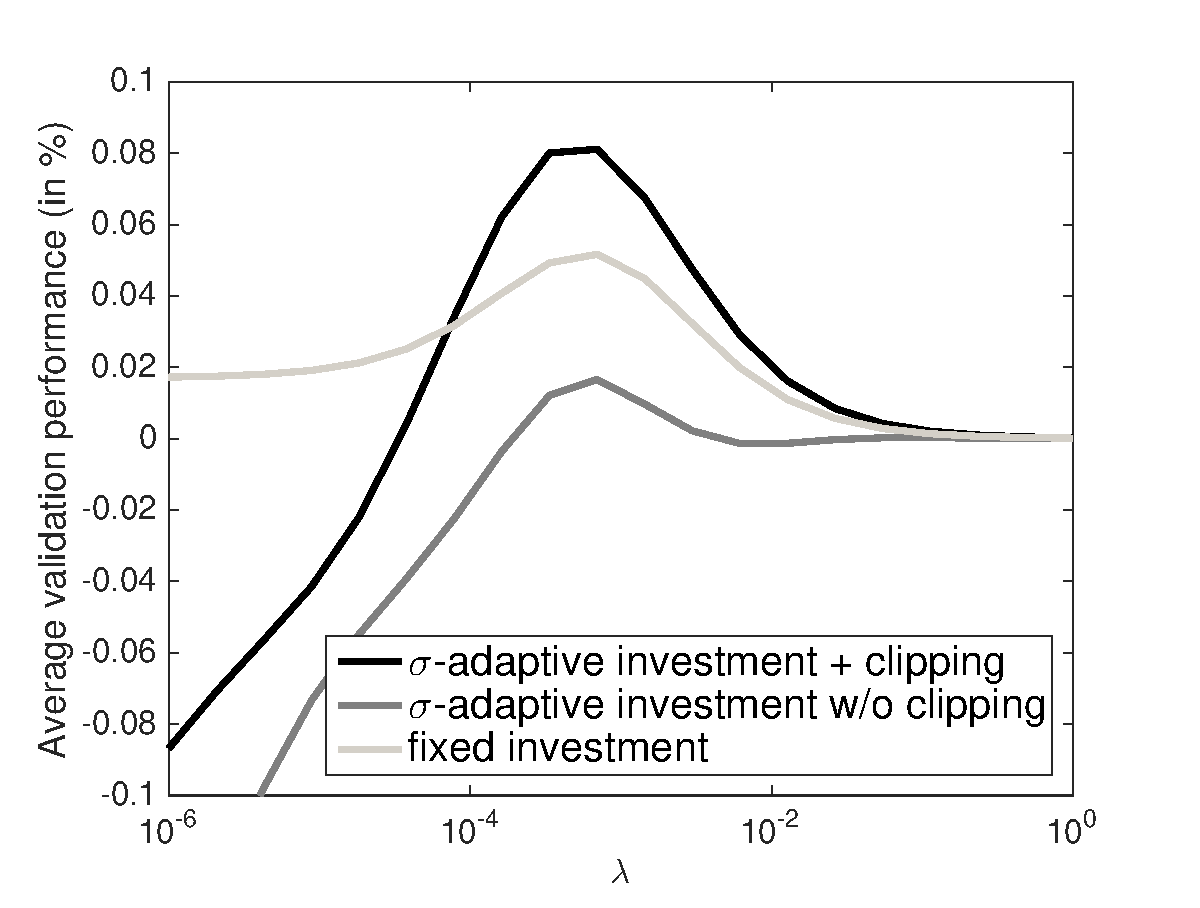
\includegraphics[width=\linewidth]{crossValidate.eps}
	\mbox{(a)}
\end{minipage}
\hfill
\begin{minipage}[t]{0.45\linewidth}
	\centering
	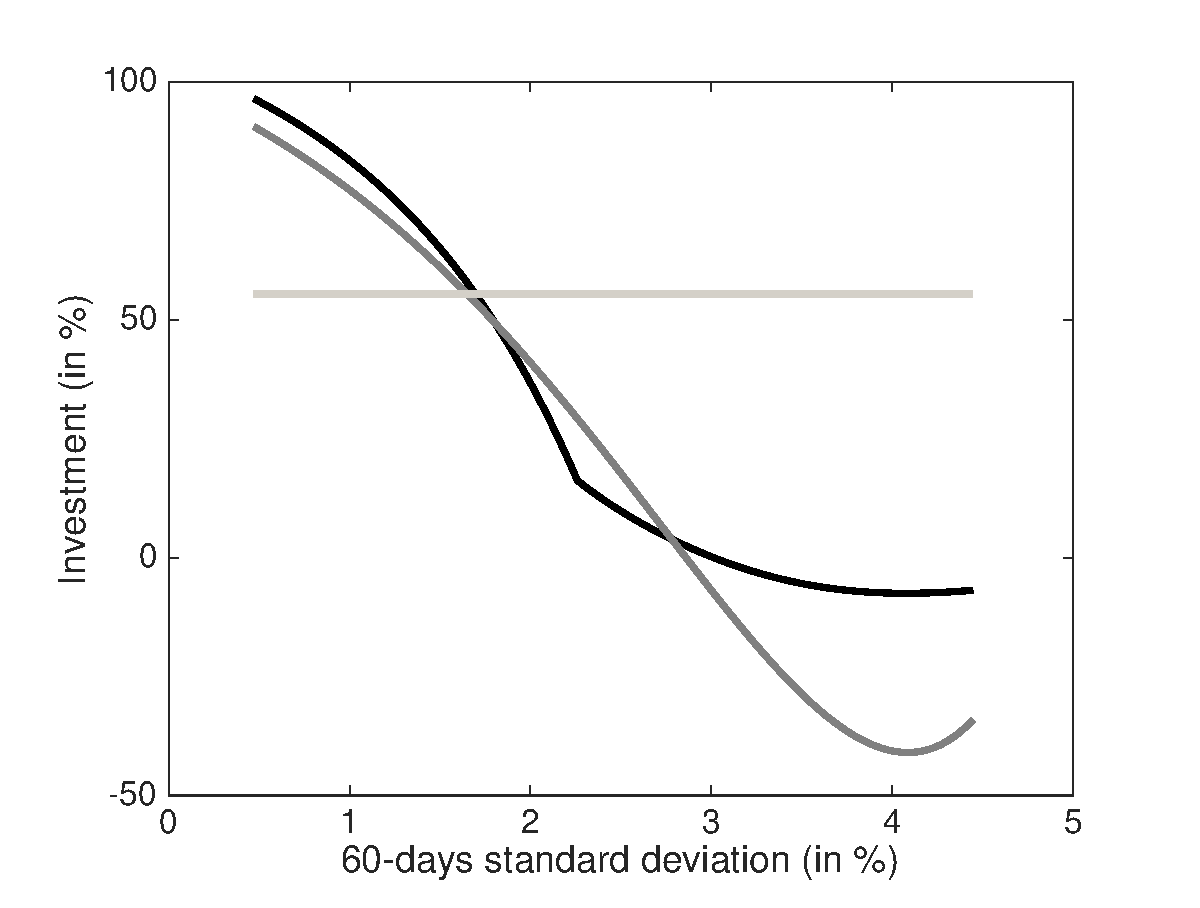
\includegraphics[width=\linewidth]{Policy.eps}
	\mbox{(b)}
\end{minipage}%
\caption{Comparison of three forms of trained investment policies. (a) presents the average performance of each policy for different values of $\lambda$ on randomly generated validation sets. (b) presents the structure of each investment policies trained using the $\lambda$ that performed best during validation.}
\label{fig:crossvalidate}
\end{figure}

%discuss out of sample performance
We next present out-of-sample performance of the three policies presented in Figure \ref{fig:crossvalidate}(b). In particular, we evaluated the 257 weekly returns achieved in the period ranging from 2014 to 2018. Considering each weekly return as an equiprobable outcome of the performance of the policies out-of-sample, it is possible to evaluate the certainty equivalent of the out-of-sample performance. Specifically, the \adaptPclipped{} achieved an out-of-sample performance of 0.16\% (8.77\% yearly), while the regular  \adaptPstd{} and \fixedP{} achieved an out-of-sample performance of   0.15\% (8.29\% yearly) and  0.12\% (6.40\% yearly) respectively. One can remark that the effect of clipping is not as apparent here given that the 60-days standard deviation in the test data ranged from 0.4\% to 1.5\% perhaps due to the absence of a recession during this period. This is a region of volatility for which both trained policies were somewhat similar (see Figure \ref{fig:crossvalidate}(b)). The poor performance of the \fixedP{} can be explained by its over-conservatism. Indeed, since the training period included the financial crisis of 2007-2008, we have as a result that the \fixedP{} recommends to cautiously invest only 56\% of the wealth in the index fund. On the other hand, $\sigma$-adapted policies were able to learn to protect the investor by reducing the investment when the volatility is large while making sure to seize the opportunities in markets that are more stable. 

For completeness, while our policies are not designed for dynamic management, we also present in Figure \ref{fig:growth}(a) the amount of wealth that would be cumulated by each policy if they were to be implemented every week during the period spanning from 2014 to 2018. The figure also presents in (b) and (c) respectively the computed 60-days standard deviation and the recommended investments for the same period. One can observe in this figure how an increase in volatility as a direct effect on reducing the investment sometime by as much as 30\%. Finally, we note that the question of how to properly train a dynamic investment policy that exploits market side information is left for future work.

\begin{figure}[h]
\begin{centering}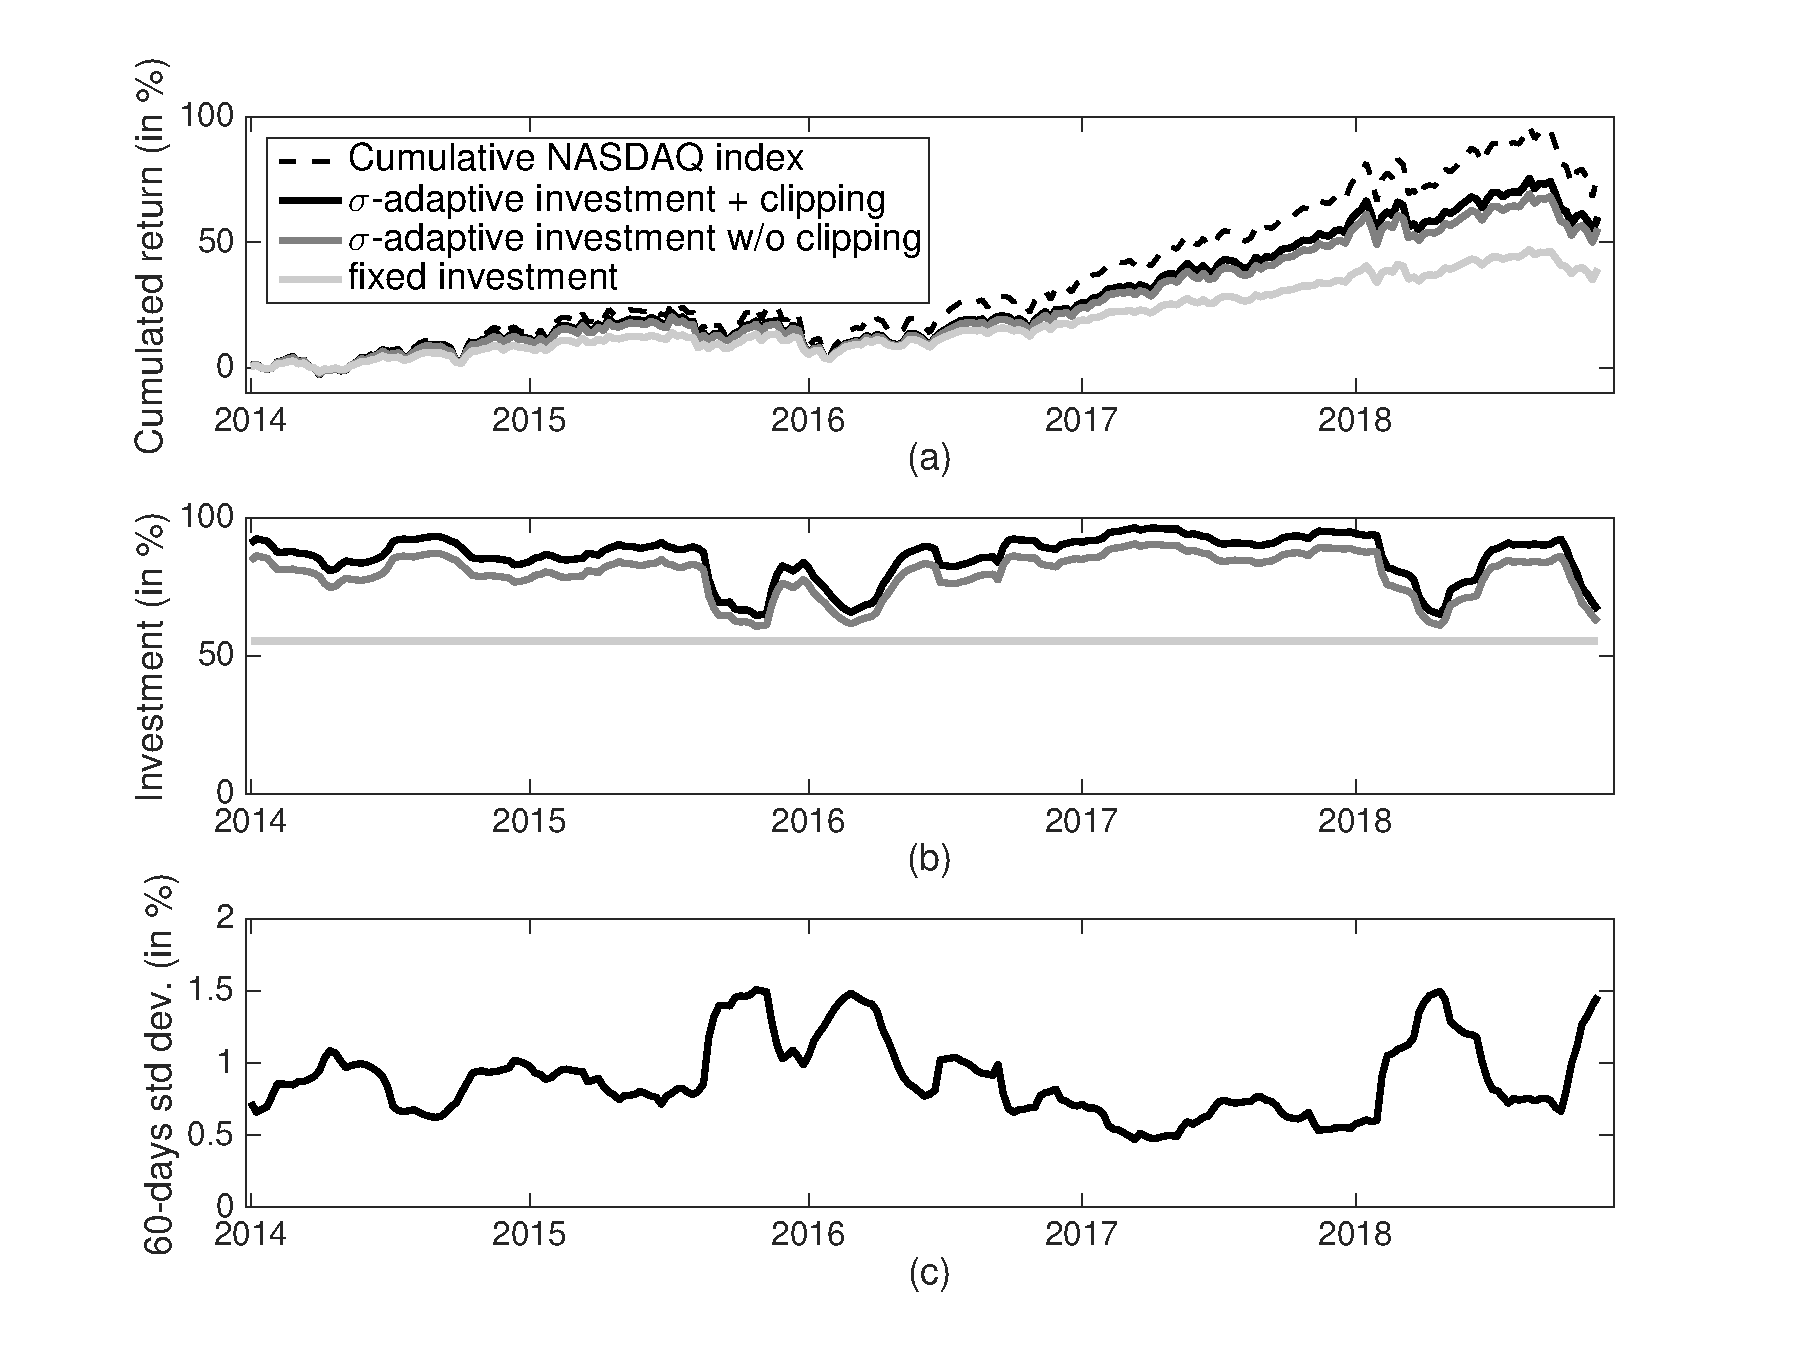
\includegraphics[width=1\columnwidth]{InvestmentGrowth}
\end{centering}
\caption{Comparison of investment strategies obtained from three trained investment policies in out-of-sample period of 2014 to 2018. (a) presents the evolution of cumulated wealth for each strategy. (b) presents the weekly investment implemented by each strategy. (c) presents the 60-days standard deviation of the index which is exploited by the $\sigma$-adapted policies.}
\label{fig:growth}
\end{figure}

%discuss generalization error 
We close this section with a discussion on how the theoretical generalization error bound and subotpimality bound established in theorems \ref{thm:outsampleBound1} and \ref{thm_truopt} compare to some evidence provided by this case study. In this regard, we revisit the 30 pairs of training and validation sets generated using bootstrapping to estimate empirical versions of these bounds. Based on construction, for the \adaptPclipped{}, we have that  $\bar{r}=2.9\%$, $\xi=2$, $\gamma=1$, and $\lambda=6.95\times10^{-4}$. We also choose to set $\delta=0.1$, and to assume that $\|q^*\|_2^2\leq 13$ based on the average norm of optimal policies in the validation data sets. Figure \ref{fig:generalizationError}(a) presents both the theoretical generalization error bound and the empirical bound (i.e. the $1-\delta$ quantile of generalization error on validation sets). Figure \ref{fig:generalizationError}(b) does the same for suboptimality gap. In both case, a monomial is fitted to the empirical bounds to indicate the order of the decay. Looking more closely at Figure \ref{fig:generalizationError}(a) we can see that the empirical error seems to decrease at a rate proportional to $n^{-0.93}$ which is closer to $O(n^{-1})$ than $O(n^{-0.5})$ and could indicate that the constant in the second term of the definition of  $\Omega_1$ might be more conservatively estimated than needed. Regarding Figure \ref{fig:generalizationError}(a), we see that the empirical rate of suboptimality reduction is of the order of $n^{-0.39}$ which is not below the rate of $O(n^{-0.5})$ and might indicate that$n$ is of a size at which $\lambda$ needs to be decreased in order to further reduce the gap.

\begin{figure}[h]
\begin{minipage}[t]{0.45\linewidth}
	\centering
	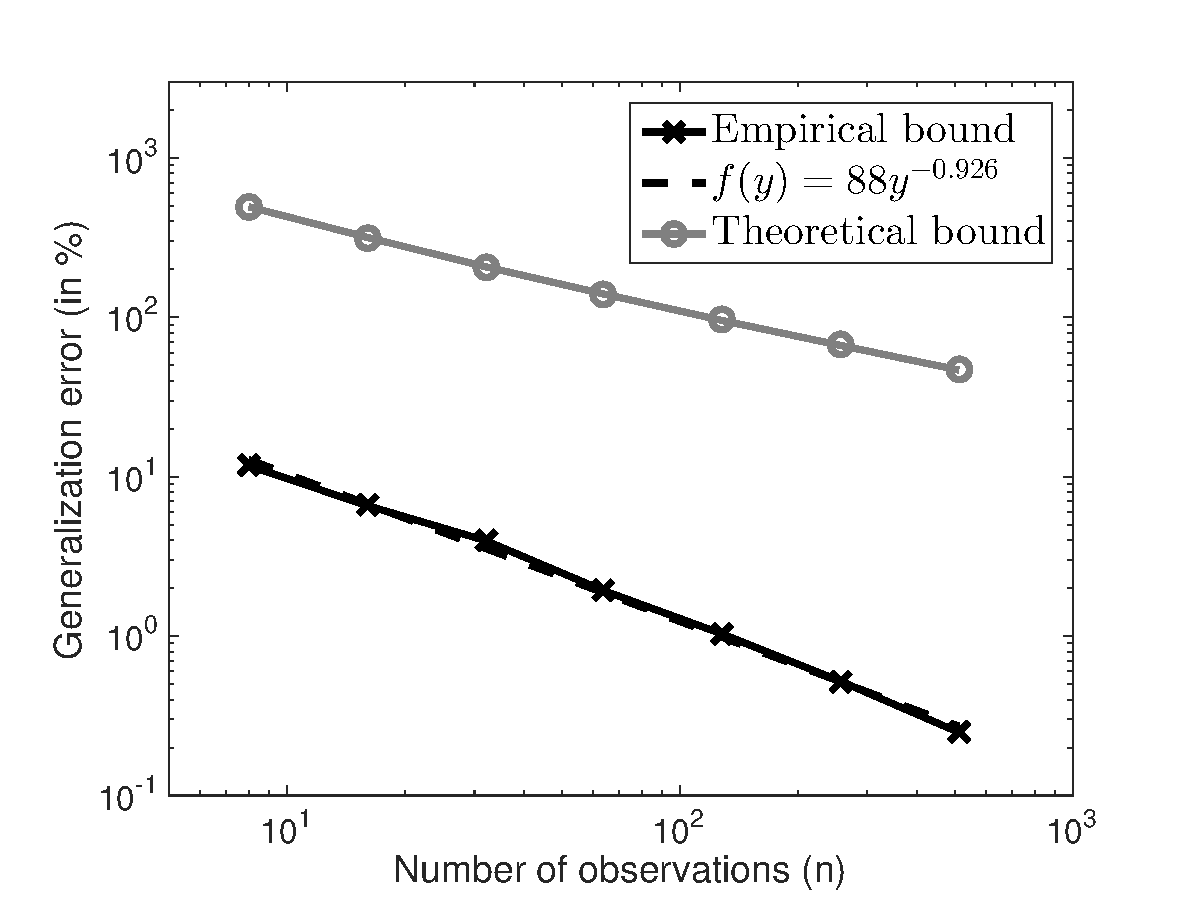
\includegraphics[width=\linewidth]{genError.eps}
	\mbox{(a)}
\end{minipage}
\hfill
\begin{minipage}[t]{0.45\linewidth}
	\centering
	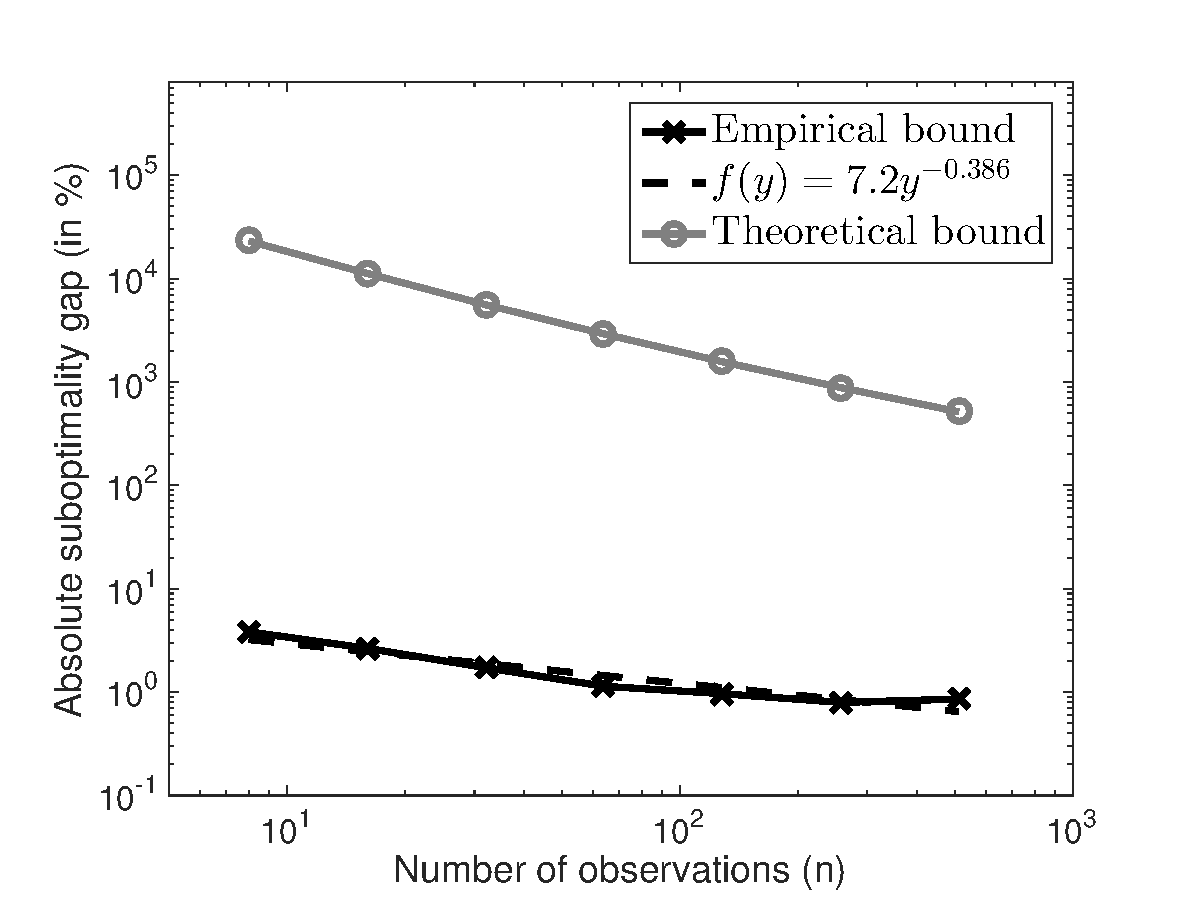
\includegraphics[width=\linewidth]{suboptError.eps}
	\mbox{(b)}
\end{minipage}%
\caption{Comparison of empirical and theoretical bounds on generalization error in (a) and suboptimality gap in (b). Both figures also present the monomial equation that best fits the empirical data.}
\label{fig:generalizationError}
\end{figure}


%\input{conclusion}
\section{\modified{Discussion}}\label{sec:conc}

As a conclusion, we would like to review the main messages we hope to deliver with this
paper. First off, as illustrated in Section \ref{sec:num} it can be very useful to use side information about financial markets, such as volatility measures, market
news, financial indicators, economic variables and so on in order to build portfolios of single or multiple risky assets. More importantly, when this is done using the regularized empirical expected utility maximization problem \eqref{EUFhatReg}, we established that, under mild conditions, a solution comes with statistical guarantees regarding its out-of-sample performance. One also has statistical guarantees on the suboptimality of the empirical decision in comparison to what might have been the best decision, given full knowledge of the market distribution.  These guarantees can be used to establish the statistical consistency of problem \eqref{EUFhatReg}  (i.e. the convergence to a truly optimal solution as $n$ goes to infinity)  when $\omega(\sqrt{n}/p)\leq \lambda \leq o(1)$ for the single asset problem.  

Secondly, these results have natural extensions for the case where the space of investment strategies is defined using kernel operators. In particular, it appears that radial basis function kernels become especially effective in a big data regime (i.e. the dimensionality of the feature vector grows with $n$)  given that the performance guarantees for this family of kernel operators are unaffected by dimensionality.

Finally, while the empirical evidence that was presented in Section \ref{sec:num} seem to indicate that these performance bounds are overly conservative, we still believe that establishing these performance guarantees provide essential guidance in the design of data-driven investment policies. In particular, in our experiments the policy that was able to achieve the best out-of-sample performance, both on the validation and the test data was a policy that employed clipping of the feature vector in order to satisfy Assumption \ref{ass:X}. Looking forward, we believe that there is a need for more extensive numerical studies that would explore the strength and limitations of the modeling paradigm that is proposed in this paper. In particular, the multi-asset setting would appear especially interesting together with settings where a richer source of market side information is used to inform the portfolio. On the theoretical side, there are also interesting open questions regarding how to tighten the performance bounds or improve on them using methods proposed in \cite{soroosh2017} and \cite{Duchi2017}, and how to extend the performance guarantees to dynamic portfolio management.

\bibliographystyle{tfcse}
\bibliography{bibliography}


%\section{Appendix}
%\input{appendix2}
\section{Appendix}

%\input{thm1_proof}
\subsection{\modified{Proof of Theorem \ref{thm:outsampleBound1}}}\label{sec:thm1_proof}

In this proof, we will make use of an adapted version of a theorem made famous by \cite{bousquet2002stability} in the context of learning theory to analyse
relevant statistical properties of the investment policy $\qhat$ presented in Section \ref{sec:model}. While this theorem discusses the use of a learning algorithm, we will rather refer to an investment algorithm which is defined next.
\begin{definition}
  Let a investment algorithm $\investA:\Re^{(p+1)\times n}\times \Re^p \rightarrow \Re$ be a procedure that generates a portfolio recommendation based on a historical sample set
  $\Sn:=\{(x_i,r_i)\}_{i=1}^n$, where each $x_i\in\Sx$ and each $r_i\in \Sr$,  and the current market conditions $x$, in other words, it produces the recommendation of investing $\investA(\Sn,x)$ in the risky asset and $1-\investA(\Sn,x)$ in the risk-free asset.
\end{definition}

We start by adapting Theorem 11.1 from \cite{mohri2012foundations} (originally found in \cite{bousquet2002stability}) to our context. To do so, we need to adapt the concept of $\beta-stability$ to the case of investment algorithms.
\begin{definition}
A investment algorithm $\investA(\cdot)$ is uniformly $\beta$-stable if for any two sample sets
  $\Sn^1:=\{(x_i^1,r_i^1)\}_{i=1}^n$ and $\Sn^2:=\{(x_i^2,r_i^2)\}_{i=1}^n$ that are
  exactly identical except for the $j$-th sample, i.e., $(x_i^1,r_i^1)=(x_i^2,r_i^2)$ for
  all $i\neq j$, the following holds:
  \[
    |u(r\,\investA(\Sn^1, x)) - u(r\,\investA(\Sn^2,x))| \leq \beta\,,\,\forall\,x\in\Sx\,,\,\forall\,r\in\Sr\;.
  \]
\end{definition}

We also introduce an additional property of the  investment algorithm which will be used instead of the notion of bounded loss for learning algorithms since, unlike loss functions, utility functions are typically neither bounded above nor below.
\begin{definition}
An investment algorithm $\investA$ achieves a $\Delta$-bounded utility range if for all sample sets $\Sn^1$ and $\Sn^2$, we have that
\[     |u(r\,\investA(\Sn^1, x))-u(r'\,\investA(\Sn^2, x'))| \leq \Delta\,,\,\forall (r,x)\in\Sr\times \Sx,\,\forall(r',x')\in\Sr\times\Sx\,.\]
\end{definition}


\begin{thm}[First adapted version of Theorem 11.1 in \cite{mohri2012foundations}]\label{thm:thm111}
  Given that  an investment algorithm $\qhat(\cdot)$ is uniformly $\beta$-stable and achieves a $\Delta$-bounded utility range, then one
  is guaranteed with a confidence of $1-\delta$ that
  \[
    \Expect_{\F}[u(R\cdot\investA(\Sn,X))] \geq \Expect_{\hat\F}[u(R\cdot\investA(\Sn,X))] - \beta -
    \left(2n\beta+\Delta\right)\sqrt{\frac{\ln(1/\delta)}{2n}}\;.
  \]
\end{thm}

The proof of this theorem follows exactly the same steps as the proof proposed in \cite{mohri2012foundations} except that the $\Delta$-bound is used to bound the expression $ |u(r\,\investA(\Sn^1, x)) - u(r'\,\investA(\Sn^2,x'))| $ instead of using upper and lower bounds for $u(\cdot)$ over its entire domain.

We now have in hand the necessary tools to obtain the result presented in Theorem \ref{thm:outsampleBound1} by considering the investment algorithm defined as $\investA(\Sn,x):=\qhat(\Sn)^T x$
where $\qhat(\Sn):=\argmax_q \;\;\;\Expect_\Fhat[u(R\cdot q^TX)]+\lambda\|q\|_2^2$. In particular, we will be interested in identifying the $\beta$-stability and the $\Delta$-bound for this estimator

\begin{lemma}\label{beta-bound}
  When assumptions \ref{ass:R}, \ref{ass:X} and \ref{ass:u} are satisfied, the investment algorithm $\investA(\cdot)$
 is uniformly $\beta$-stable with  $ \beta = \frac{(\gamma\bar r\xMax)^2}{2\lambda n}$. 
\end{lemma}

\begin{proof}
We first establish that for any
  pair $(q_1,q_2)\in\Re^p\times\Re^p$, one has that
  \[ 
    |u(r\,q_1^T x) - u(r\,q_2^T x)| \leq \gamma |rq_1^Tx - rq_2^Tx|\leq \gamma|r|\|x\|_2\|q_1- q_2\|_2 \leq \gamma\bar{r} \xi \|q_1- q_2\|_2\,,\,\forall\,r\in\Sr\,,\,\forall\,x\in\Sx\;.
  \]
  This follows naturally from Assumption \ref{ass:u} which states that $u(\cdot)$ is Lipschitz continuous, and assumptions \ref{ass:R} and \ref{ass:X}. Next, we can employ similar steps as in the proof of Proposition 11.1 from \cite{mohri2012foundations} to establish that $\|\qhat(\Sn^1)-\qhat(\Sn^2)\|_2 \leq \gamma \bar{r} \xi/(\lambda n)$ which would complete our proof since for all $x\in\Sx$ and all $r\in\Sr$, we would have that
  \[ |u(r\,\qhat(\Sn^1)^T x) - u(r\,\qhat(\Sn^2)^T x)| \leq \gamma\bar{r} \xi \|\qhat(\Sn^1)- \qhat(\Sn^2)\|_2 \leq \gamma^2 \bar{r}^2\xi^2 /(\lambda n)\]
  
To summarize how   $\|\qhat(\Sn^1)-\qhat(\Sn^2)\|_2 \leq \gamma \bar{r} \xi/(\lambda n)$ is obtained, we first observe that since $\qhat(\Sn^1)$ is the maximizer of the concave function $\widehat{EU}_{\Sn^1}(q)-\lambda \|q\|_2^2$ where $\widehat{EU}_{\Sn}(q):=(1/n)\sum_{i=1}^n u(r_i q^T x_i)$, there must exist a super-gradient equal to zero at $\qhat(\Sn^1)$. In particular, there must be a super-gradient $\nabla\widehat{EU}_{\Sn^1}(\qhat(\Sn^1))$ of $\widehat{EU}_{\Sn^1}(q)$ at $\qhat(\Sn^1)$ such that 
\[\nabla\widehat{EU}_{\Sn^1}(\qhat(\Sn^1))-2\lambda \qhat(\Sn^1) = 0\;\;\Rightarrow\;\;\nabla\widehat{EU}_{\Sn^1}(\qhat(\Sn^1))=2\lambda \qhat(\Sn^1)\,.\]
Together with the concavity of $\widehat{EU}_{\Sn^1}(q)$, this implies that
\begin{align*}
\widehat{EU}_{\Sn^1}(\qhat(\Sn^2))&\leq \widehat{EU}_{\Sn^1}(\qhat(\Sn^1)) + \nabla\widehat{EU}_{\Sn^1}(\qhat(\Sn^1))(\qhat(\Sn^2)-\qhat(\Sn^1))\\
&=\widehat{EU}_{\Sn^1}(\qhat(\Sn^1)) + 2\lambda \qhat(\Sn^1)^T(\qhat(\Sn^2)-\qhat(\Sn^1))\,
\end{align*}
and similarly that
\begin{align*}
\widehat{EU}_{\Sn^2}(\qhat(\Sn^1))\leq \widehat{EU}_{\Sn^2}(\qhat(\Sn^2)) + 2\lambda \qhat(\Sn^2)^T(\qhat(\Sn^1)-\qhat(\Sn^2))\,.
\end{align*}
Together, these two inequalities can be used to conclude that 
\begin{align*}
2\lambda &\|\qhat(\Sn^2)-\qhat(\Sn^1)\|_2^2 \;=\; 2\lambda \qhat(\Sn^2)^T(\qhat(\Sn^2)-\qhat(\Sn^1)) - 2\lambda \qhat(\Sn^1)^T(\qhat(\Sn^2)-\qhat(\Sn^1))\\
&\leq\; \widehat{EU}_{\Sn^1}(\qhat(\Sn^1)) -  \widehat{EU}_{\Sn^1}(\qhat(\Sn^2)) + \widehat{EU}_{\Sn^2}(\qhat(\Sn^2)) - \widehat{EU}_{\Sn^2}(\qhat(\Sn^1))\\
&=\; (1/n)(u(r_m^1 \qhat(\Sn^1)^Tx_m^1)-u(r_m^1 \qhat(\Sn^2)^Tx_m^1) + u(r_m^2 \qhat(\Sn^2)^Tx_m^2)-u(r_m^2 \qhat(\Sn^1)^Tx_m^2)\\
&\leq\; (2\gamma \bar{r}\xi/n)\|\qhat(\Sn^2)-\qhat(\Sn^1)\|_2\,,
\end{align*}
where the second equality comes from the definition of $\widehat{EU}_{\Sn}$ and the second inequality follows from assumptions \ref{ass:R}, \ref{ass:X}, and \ref{ass:u}. By dividing both sides of the inequality by $2\lambda\|\qhat(\Sn^2)-\qhat(\Sn^1)\|_2$ we get our stated property.
\end{proof}

\begin{lemma}\label{u-bound}
  When assumptions \ref{ass:R}, \ref{ass:X} and \ref{ass:u} are satisfied, the $\Delta$-bound on the utility range for $\investA(\cdot)$ is $\Delta:= \frac{(\gamma+1)\xi^2
      \bar{r}^2}{2\lambda}$.
\end{lemma}

\begin{proof}
  This proof relies mostly on demonstrating that $\|\qhat(\Sn)\|_2\leq \bar{r}\xi/(2\lambda)$
  with probability one with respect to the randomness of $\Sn$. Indeed, when this is the case,
  then we have that
  \begin{align*}
    |u(r_1\,\qhat(\Sn^1)^T x_1)-u(r_2\,\qhat(\Sn^2)^T x_2)| &\;\leq\; u(\bar{r}^2\xi^2/(2\lambda) )-u(- \bar{r}^2\xi^2/(2\lambda))\\
    &\modified{\;\leq\;|u(\bar{r}^2\xi^2/(2\lambda) )-u(0)|+|u(0)-u(-\bar{r}^2\xi^2/(2\lambda))|}\\
    &\;\leq\; (1+\gamma)\bar{r}^2\xi^2/(2\lambda)     \;.
  \end{align*}
  In order to identify a bound on the norm of $\qhat(\Sn)$, we reformulate problem
  \eqref{EUFhatReg} as follows
  \begin{eqnarray*}
    \maximize_{s\in\Re,v\in\Re^p} && \frac{1}{n}\sum_{i=1}^n u(s R_i\,X_i^T v) - \lambda s^2\\
    \subto&& s\geq0\;,\;\|v\|_2=1\;,
  \end{eqnarray*}
  such that $\qhat(\Sn) =s^*\cdot v^*$ when $(s^*,v^*)$ is the pair of optimal
  assignments for this optimization problem. It is therefore clear that
  $s^*=\|\qhat(\Sn)\|_2$ and our proof reduces to establishing an upper bound for $s^*$.
  By recognizing that
  $s^*=\argmax_{s\geq 0} g(s):=\frac{1}{n}\sum_{i=1}^n u(s R_i\,X_i^T v^*) - \lambda s^2$
  and that $g(s)$ is a concave function, then it is necessarily the case that if there
  exists a $\bar{s}\geq 0$ such that $g(\cdot)$ is non-increasing at $\bar{s}$ then
  $s^* \leq \bar{s}$. We can actually show that this is the case for
  $\bar{s}:= \bar{r}\xi/(2\lambda)$ by upper bounding the impact of taking a step of
  $\delta>0$:
  \begin{eqnarray*}
    g(\bar{s}+\delta)-g(\bar{s}) &=& \frac{1}{n}\sum_{i=1}^n (u((\bar{s}+\delta) R_i\,X_i^T v^*) - u(\bar{s} R_i\,X_i^T v^*) ) - \lambda ((\bar{s}+\delta)^2-\bar{s}^2)\\
                                 &\leq& \frac{1}{n}\sum_{i=1}^n (u((\bar{s}+\delta) |R_i\,X_i^T v^*|) - u(\bar{s} |R_i\,X_i^T v^*|) ) - \lambda ((\bar{s}+\delta)^2-\bar{s}^2)\\
                                 &\leq & \frac{1}{n}\sum_{i=1}^n  \delta |R_i\,X_i^T v^*| - \lambda (2\bar{s}\delta + \delta^2)\\
                                 &\leq &  \delta \bar{r} \xi  - 2\lambda \bar{s}\delta -  \delta^2 = -  \delta^2 \leq 0\;,
  \end{eqnarray*}
  where we first used the fact that $u(\cdot)$ is increasing, next that
  $u(y+\delta)\leq u(y)+\delta$ when $\delta\geq 0$ since it is a concave function with a
  subgradient of one at zero.  Finally, we exploited assumptions \ref{ass:R} and
  \ref{ass:X} and used the definition of $\bar{s}$. This completes our proof.
\end{proof}

We have therefore established that under assumptions \ref{ass:R}, \ref{ass:X}, and \ref{ass:u}, we have that
\begin{eqnarray}
    \Expect_{\F}[u(R\cdot\investA(\Sn,X))] \geq \Expect_{\hat\F}[u(R\cdot\investA(\Sn,X))] - \Omega_1\;.\label{app:eq:genBoundUtil}
\end{eqnarray}
 We can now conclude this section by demonstrating how Theorem \ref{thm:outsampleBound1} follows
from this fact. In particular, by concavity of the utility
function, we have that
\[
  u(\CE(\qhat;\F))\leq u(\CE(\qhat;\Fhat))+(\CE(\qhat;\F)-\CE(\qhat;\Fhat))\,\nabla
  u(\CE(\qhat;\Fhat))\;,
\] 
where $\nabla u(r)$ denotes any supergradient of $u(\cdot)$ at $r$. In particular, since
$u(\cdot)$ is an increasing concave function, it follows that
$\lim_{\epsilon\to0^-}u'(\CE(\qhat;\Fhat)+\epsilon)\geq 0$ is one of the supergradient at
$\CE(\qhat;\Fhat)$. Combining this inequality with the inequality presented in equation \eqref{app:eq:genBoundUtil}, we get
\begin{align*}
  u(\CE(\qhat;\Fhat)) - \Omega_1 &=  \Expect_{\hat\F}[u(R\cdot\investA(\Sn,X))] - \Omega_1 \leq   \Expect_{\F}[u(R\cdot\investA(\Sn,X))] \\
  &= u(\CE(\qhat;\F)) \leq
  u(\CE(\qhat;\Fhat))+(\CE(\qhat;\F)-\CE(\qhat;\Fhat))\nabla u(\CE(\qhat;\Fhat))
\end{align*}
so that
\[
  \CE(\qhat;\F) \geq \CE(\qhat;\Fhat) - \Omega_1/\nabla u(\CE(\qhat;\Fhat))
\]
follows since it was assumed that $u(\cdot)$ is strictly increasing. This completes the
proof of Theorem \ref{thm:outsampleBound1}. \Halmos



%\input{thm2_proof}
\subsection{\modified{Proof of Theorem \ref{thm_truopt}}}\label{app:thm_truopt}

We first show that there exist an optimal solution $q^*$ for problem \eqref{EUF}.

\begin{lemma}\label{thm:qstarBound}
Given assumptions \ref{ass:R}, \ref{ass:X}, and \ref{ass:arbitrage}, we have that problem \eqref{EUF} is bounded.
\end{lemma}

\begin{proof}
Similarly as was done in the proof of Lemma \ref{u-bound}, we can reformulate problem \eqref{EUF} in terms of both  an orientation vector and a scale decision variable. This gives us
  \begin{eqnarray*}
    \maximize_{s\in\Re,v\in\Re^p} && \Expect_F[ u(s R\,X^T v)] \\
    \subto&& s\geq0\;,\;\|v\|_2=1\;.
  \end{eqnarray*}
Note that the optimal value of the above problem is necessarily greater or equal to $u(0)=0$. Moreover, in the case where it is exactly zero, then $s^*=0$ is an optimal solution and we can conclude that there exists a bounded $q^*$. We therefore focus in what follows on the case where the optimal value is strictly positive or even unbounded.

Based on Assumption \ref{ass:arbitrage}, since no feature induces an arbitrage opportunity, it follows that
for any $v$ of norm equal to one, either $\Prob_F(RX^Tv=0)=1$ or there exists a $\delta>0$ and a $\varrho>0$ such that $\Prob_F(R\,X^T v<-\delta)=\varrho$ . In the former case, $v$ cannot be an optimal assignment since $\Expect_F[ u(s R\,X^T v)] = u(0)$ for all $s\geq 0$ which we assumed was a sub-optimal objective value.  Now, in the latter case,
we let $B$ be a discrete random variable with two states such that
$\Prob_F(B=-\delta)=1-\Prob_F(B=\bar r\xi)=\varrho$. Since $|R\,X^T v|\leq \bar r\xi$, we have
that $\Prob_F(B\geq r) \geq \Prob_F(R\,X^T v\geq r)$ for all $r\in\Re$, i.e. that $B$ stochastically dominates $R\,X^T v$, so that 
it must necessarily follow that $\Expect_F[u(sB)]\geq \Expect_F[u(sR\,X^T v)]$ for all $s\geq 0$. But, by the sublinearity asumption on
$u$,
\begin{align*}
  \lim_{s\to\infty}\Expect_F[u(sR\,X^T v)] &\leq   \lim_{s\to\infty}\Expect_F[u(sB)]  = \lim_{s\to\infty}\big(\varrho  u(-s\delta)+(1-\varrho)u(s\bar r\xi)\big) \\
  &\leq   \lim_{s\to\infty} -\varrho s\delta + (1-\varrho) o(s) =  -\infty\;
 \end{align*} 
%\[
%  \lim_{s\to\infty}\Expect_F[u(sB)] = \lim_{s\to\infty}\big(\varrho
%  u(-s\delta)+(1-\varrho)u(s\bar r\xi)\big) \leq   \lim_{s\to\infty} -\varrho s\delta + (1-\varrho) o(s) =  -\infty\;
%\]
which shows that
$s^\star$, and therefore $\|q^\star\|_2$, is bounded.
\end{proof}

We next invoke a theorem from \cite{sridharan2009fast} which will be of use.

\begin{thm}[See Theorem 1 in \cite{sridharan2009fast}]\label{thm:sridharan}
Let $\mathcal{W}$ be a closed convex subset of a Banach space with norm $\|\cdot\|$ and dual norm $\|\cdot\|_*$ and consider $f(w,x,r):= \ell(\langle w, \Phi(x,r)\rangle;x,r) +\lambda\|w\|^2$, where $\ell:\Re\times\Re^{p+1}\rightarrow\Re$ is $L$-Lipschitz and convex in its first argument and where $\Phi:\Re^{p}\times\Re\rightarrow \mathcal{W}$ is bounded such that $\Prob_F(\|\Phi(X,R)\|\leq B)=1$. Then, for any $\delta>0$, with probability at least $1-\delta$ over a sample of size $n$, we have that :
\[F(\hat{w})-F(w^*)\leq \frac{4 L^2 B^2(32+\ln(1/\delta)}{\lambda n}\,,\]
where $F(w):=\Expect_F[f(w,X,R)]$, $\hat{F}(w):=(1/n)\sum_{i=1}^n f(w,x_i,r_i)$, $w^* := \argmin_{w\in\mathcal{W}}  F(w)$, and $\hat{w}:= \argmin_{w\in\mathcal{W}} \hat{F}(w)$.
\end{thm}

By considering that $\Phi(x,r):=x$, which is bounded by $\xi$ when using the 2-norm, and that $\ell(z;x,r):=-u(zr)$ which is convex and $\gamma \bar{r}$-Lipschitz for all $x\in\Sx$ and $r\in\Sr$, we immediately get the following corollary. Note that to get this result we also exploit the fact that $f(q,x,r)$ is $2\lambda$-strongly convex with respect to the 2-norm which implies, based on for example Lemma 13 in \cite{ShalevThesis} that : $F(\hat{w})\geq F(w^*)+\lambda\|\hat{w}-w^*\|_2^2$.
 
\begin{corollary}\label{thm:shai}
  Given that assumptions \ref{ass:R}, \ref{ass:X}, and \ref{ass:u} are satisfied, then one has with confidence of
  $1-\delta$ that
  \[
    -\lambda\|\hat q - q^\star_\lambda\|_2^2 \geq \EU_\lambda(\hat q) - \EU_\lambda(q^\star_\lambda) \geq -\omega,
  \]
  where $\omega := 4\gamma^2\bar{r}^2 \xi^2(32+\ln(1/\delta))/(\lambda n)$ and  $\EU_\lambda(q) := \Expect_F(u(R\cdot q^T X)) - \lambda\|q\|_2^2$,
with $q^\star := \argmin_q \EU(q)$ and $q^\star_\lambda := \argmin_q \EU_\lambda(q)$.
\end{corollary}

Notice that Corollary \ref{thm:shai} implies with confidence $1-\delta$ that
\[
  \EU(\hat q) - \EU(q^\star_\lambda) \geq \lambda\bigl(\|\hat q\|_2^2 -
  \|q^\star_\lambda\|_2^2\bigr) -\omega
  \geq -\lambda\bigl(\|\hat q -
  q^\star_\lambda\|_2^2 +2\|\qhat\|_2\|\qhat  - q^\star_\lambda\|_2\bigr) - \omega.
\]
where $\EU(\qhat) := \Expect_F(u(R\cdot \qhat^T X))$. As shown in Lemma \ref{u-bound}, $\|\qhat\|_2 \leq \bar r\xi/(2\lambda)$. Hence, Theorem \ref{thm:shai} further implies concerning the same $1-\delta$ probability outcomes that
$\|\hat q - q^\star_\lambda\|_2^2 \leq \omega/\lambda$, and therefore
$\|\hat q - q^\star_\lambda\|_2 \leq \sqrt{\omega/\lambda}$, so that we end up with
\[
  \EU(\hat q) - \EU(q^\star_\lambda) \geq -2\omega - \bar r\xi\sqrt{\frac{\omega}{\lambda}}.
\]
with probability $1-\delta$. Finally, note that since by the  definition of $q^\star_\lambda$, we have that
\[
  \EU(q^\star) - \lambda\|q^\star\|_2^2 \leq \EU(q^\star_\lambda) - \lambda\|q^\star_\lambda\|_2^2\;,
\]
it follows that
\[
  \EU(q^\star) - \EU(q^\star_\lambda) \leq \lambda\bigl(\|q^\star\|_2^2 -
  \|q^\star_\lambda\|_2^2\bigr) \leq \lambda\|q^\star\|_2^2,
\]
so that we can bound the suboptimality of the policy $\hat q$ with probability $1-\delta$
in the following fashion:
\begin{align*}
  \EU(\hat q) &= \EU(q^\star) + \EU(\hat q) - \EU(q^\star_\lambda) + \EU(q^\star_\lambda)
                - \EU(q^\star)\\
              &\geq \EU(q^\star) - 2\omega - \bar r\xi\sqrt{\frac{\omega}{\lambda}}  - \lambda\|q^\star\|_2^2 =  \EU(q^\star) - \Omega_2.
\end{align*}
This relation can be exploited in a similar way as in the proof of Theorem \ref{thm:outsampleBound1} (see Section \ref{sec:thm1_proof}) to derive the relation between certainty equivalents that is presented in our theorem. \Halmos




\subsection{\modified{Proof of Theorem \ref{thm:outsampleBound1:Multi}}}\label{sec:thm1_proofMulti}
\newcommand{\vinvestA}{{\boldsymbol{\pi}}}

This proof follows exactly the same steps as the proof of Theorem \ref{thm:outsampleBound1}. Namely, we can exploit another adapted version of Theorem 11.1 in \cite{mohri2012foundations} for a multi-asset investment algorithm $\vinvestA:\Re^{\vp+1\times m \times n} \times \Re^\vp \rightarrow \Re^m$ which constructs an investment portfolio based on a training set $\Sn:=\{(\vx_1,\vr_1),\dots,(\vx_m,\vr_m)\}$, where each $\vx_i \in \Re^{m\times p}$ and each $\vr_i\in\Re^m$,  and the current market side-information matrix $\vx$. The natural extension of $\beta$-stability and $\Delta$-bound to this context is described in what follows.

\begin{definition}
A multi-asset investment algorithm $\vinvestA(\cdot)$ is uniformly $\beta$-stable if for any two sample sets
  $\Sn^1:=\{(\vx_i^1,\vr_i^1)\}_{i=1}^n$ and $\Sn^2:=\{(\vx_i^2,\vr_i^2)\}_{i=1}^n$ that are
  exactly identical except for the $j$-th sample, i.e., $(\vx_i^1,\vr_i^1)=(\vx_i^2,\vr_i^2)$ for
  all $i\neq j$, the following holds:
  \[
    |u(\vr^T\vinvestA(\Sn^1, \vx)) - u(\vr^T\vinvestA(\Sn^2,\vx))| \leq \beta\,,\,\forall\,\vx\in\vSx\,,\,\forall\,r\in\vSr\;.
  \]
\end{definition}

\begin{definition}
A multi-asset investment algorithm $\vinvestA(\cdot)$ achieves a $\Delta$-bounded utility range if for all sample sets $\Sn^1$ and $\Sn^2$:
%\[     \Prob(|u(\vr^T\vinvestA(\Sn^1, \vx))-u(\vr^T\vinvestA(\Sn^2, \vx))| \leq \Delta)=1\;.\]
\[     |u(\vr\,\vinvestA(\Sn^1, \vx))-u(\vr'\,\vinvestA(\Sn^2, \vx'))| \leq \Delta\,,\,\forall (\vr,\vx)\in\vSr\times \vSx,\,\forall(\vr',\vx')\in\vSr\times\vSx\,.\]
\end{definition}


This leads us to adapting Theorem \ref{thm:thm111} to the context of multi-asset investment algorithms.

\begin{thm}[Second adapted version of Theorem 11.1 in \cite{mohri2012foundations}]\label{thm:thm111:multi}
  Given that a multi-asset investment algorithm $\vqhat(\cdot)$ is uniformly $\beta$-stable and achieves a $\Delta$-bounded utility range, then one
  is guaranteed with a confidence of $1-\delta$ that
  \[
    \Expect_{\F}[u(\vR^T\vinvestA(\Sn,\vX))] \geq \Expect_{\hat\F}[u(\vR^T\vinvestA(\Sn,\vX))] - \beta -
    \left(2n\beta+\Delta\right)\sqrt{\frac{\ln(1/\delta)}{2n}}\;.
  \]
\end{thm}

 This time, we consider a multi-asset investment algorithm to be defined as $\vinvestA(\Sn,\vx):=\vx\vqhat(\Sn)$ where $\vqhat(\Sn):=\argmax_\vq \;\;\;\Expect_\Fhat[u(\vR^T\vX \vq)]+\lambda\|\vq\|_2^2$. In particular, the same steps can be used to verify that this algorithm is $\frac{(\gamma\bar r\xMax)^2}{2\lambda n}$-stable and that $\Delta:=\frac{(\gamma+1)\xi^2
      \bar{r}^2}{2\lambda}$ is a valid $\Delta$-bound for the utility range achieved using this estimator. For completeness, we repeat the argument that is used to establish the bound on $\vqhat(\Sn)$.

\begin{lemma}\label{thm:qhatBoundMulti}
Given assumptions \ref{ass:Rmulti} and \ref{ass:Xmulti}, we have that $\|\vqhat(\Sn)\|_2 \leq \bar{r}\xi/(2\lambda)$ with probability one.
\end{lemma}

\begin{proof}
We first reformulate problem
  \eqref{EUFhatReg} as follows
  \begin{eqnarray*}
    \maximize_{s\in\Re,\vv\in\Re^\vp} && \frac{1}{n}\sum_{i=1}^n u(s \vR_i^T \vX_i \vv) - \lambda s^2\\
    \subto&& s\geq0\;,\;\|\vv\|_2=1\;,
  \end{eqnarray*}
 such that $\vqhat(\Sn) =s^*\cdot\vv^*$ when $(s^*,\vv^*)$ is the pair of optimal
  assignments for this optimization problem. It is therefore clear that
  $s^*=\|\vqhat(\Sn)\|_2$ and our proof reduces to establishing an upper bound for $s^*$.
  By recognizing that
  $s^*=\argmax_{s\geq 0} g(s):=\frac{1}{n}\sum_{i=1}^n u(s \vR_i^T \vX_i \vv^*) - \lambda s^2$
  and that $g(s)$ is a concave function, then it is necessarily the case that if there
  exists a $\bar{s}\geq 0$ such that $g(\cdot)$ is non-increasing at $\bar{s}$ then
  $s^* \leq \bar{s}$. We can actually show that this is the case for
  $\bar{s}:= \bar{r}\xi/(2\lambda)$ by upper bounding the impact of taking a step of
  $\delta>0$:
  \begin{eqnarray*}
    g(\bar{s}+\delta)-g(\bar{s}) &=& \frac{1}{n}\sum_{i=1}^n (u((\bar{s}+\delta) \vR_i^T \vX_i \vv^*) - u(\bar{s} \vR_i^T \vX_i \vv^*) ) - \lambda ((\bar{s}+\delta)^2-\bar{s}^2)\\
                                 &\leq& \frac{1}{n}\sum_{i=1}^n (u((\bar{s}+\delta) |\vR_i^T\vX_i \vv^*|) - u(\bar{s} |\vR_i^T\vX_i \vv^*|) ) - \lambda ((\bar{s}+\delta)^2-\bar{s}^2)\\
                                 &\leq & \frac{1}{n}\sum_{i=1}^n  \delta |\vR_i^T \vX_i \vv^*| - \lambda (2\bar{s}\delta + \delta^2)\\
                                 &\leq &  \delta \bar{r} \xi  - 2\lambda \bar{s}\delta -  \lambda \delta^2 = -\lambda   \delta^2 \leq 0\;,
  \end{eqnarray*}
  where we first used the fact that $u(\cdot)$ is increasing, next that
  $u(y+\delta)\leq u(y)+\delta$ when $\delta\geq 0$ since it is a concave function with a
  subgradient of one at zero.  Finally, we exploited assumptions \ref{ass:Rmulti} and
  \ref{ass:Xmulti}. 
\end{proof}


\subsection{\modified{Proof of Theorem \ref{thm:kernelreform}}}

This follows from the representer theorem (see Theorem 9 in \cite{kernel2008}) which states that the optimal solution to problem \eqref{EUF:regKernel} always takes the form of a linear combination of the kernel expansion of the sample points. Specifically,  there exists a linear combination $\alpha \in \Re^n$ such that $\kqhat:=\sum_{j=1}^n \alpha_j \Phi(x_j)$. This implies that the optimization can be reduced to optimizing over the space of $\alpha\in\Re^n$. When doing so, the objective function becomes:
\begin{align*}
\frac{1}{n}\sum_{i=1}^n u(r_i \langle &\sum_{j=1}^n \alpha_j \Phi(x_j), \Phi(x_i)\rangle) - \lambda \langle \sum_{i=1}^n \alpha_i \Phi(x_i), \sum_{j=1}^n \alpha_j \Phi(x_j)\rangle \\
&= \frac{1}{n}\sum_{i=1}^n u(r_i \sum_{j=1}^n \alpha_j \langle \Phi(x_j), \Phi(x_i)\rangle) - \lambda \sum_{i=1}^n \sum_{j=1}^n \alpha_i  \alpha_j \langle \Phi(x_i), \Phi(x_j)\rangle\\
&= \frac{1}{n}\sum_{i=1}^n u(r_i \sum_{j=1}^n \alpha_j k(x_j,x_i)) - \lambda \sum_{i=1}^n \sum_{j=1}^n \alpha_i  \alpha_j k(x_i,x_j)\,.
\end{align*}
This directly leads to the objective function used in problem \eqref{EUF:regKernelRef}. \Halmos


\subsection{\modified{Proof of Theorem \ref{thm_truoptMulti}}}

The steps of this proof follows almost exactly as the steps presented for the proof of Theorem \ref{thm_truopt} in Appendix \ref{app:thm_truopt}. We can first demonstrate that problem \eqref{EUF} remains bounded in the multi-asset setting using the same steps as in the proof of Lemma \ref{thm:qstarBound}. We then apply Theorem \ref{thm:sridharan} using this time $\phi(\vx,\vr):=\vx^T\vr$ (instead of $\phi(x,r):=x$) , which is bounded by $\bar{r}\xi$ when using the 2-norm, and using $\ell(z;\vx,\vr):=-u(z)$ (instead of $\ell(z;x,r):=-u(zr)$) which is convex and $\gamma$-Lipschitz. Together with the fact that $f(q,\vx,\vr)$ is $2\lambda$-strongly convex with respect to the 2-norm, we immediately get the following corollary. 
 
\begin{corollary}\label{thm:shaiMulti}
  Given that assumptions \ref{ass:u}, \ref{ass:Rmulti}, and \ref{ass:Xmulti} are satisfied, then one has with confidence of
  $1-\delta$ that
  \[
    -\lambda\|\vqhat - \vq^\star_\lambda\|_2^2 \geq \EU_\lambda(\vqhat) - \EU_\lambda(\vq^\star_\lambda) \geq -\omega,
  \]
  where $\omega := 4\gamma^2\bar{r}^2 \xi^2(32+\ln(1/\delta))/(\lambda n)$ and where $\EU(\vq) := \Expect_F(u(\vR^T \vX q))$ and $\EU_\lambda(\vq) := \Expect_F(u(\vR^T \vX \vq)) - \lambda\|\vq\|_2^2$,
with $\vq^\star := \argmin_\vq \EU(\vq)$ and $\vq^\star_\lambda := \argmin_\vq \EU_\lambda(\vq)$.
\end{corollary}
The rest of the proof is straightforward and exploits the bound on $\vqhat$ established in Lemma \ref{thm:qhatBoundMulti}. \Halmos




\subsection{\modified{Proof of Theorem \ref{thm:outsampleBound1:kernel}}}\label{sec:thm1_proofKernel}

This proof follows exactly the same steps as the proof of Theorem \ref{thm:outsampleBound1} and \ref{thm:outsampleBound1:Multi}. Namely, we exploit exactly the  version of Theorem 11.1 in \cite{mohri2012foundations} presented in Theorem \ref{thm:thm111} with the investment algorithm $\investA:\Re^{p+1\times m \times n} \times \Re^p \rightarrow \Re^m$ defined as $\investA(\Sn,x):=\langle\kqhat(\Sn), \Phi(x)\rangle $. Once again, the same steps can be used, in the reproducing Hilbert kernel space $\mathcal{W}$ replacing $q$ with $\kq$ and $x$ with $\Phi(x)$ in the analysis,  to verify that this algorithm is $\frac{(\gamma\bar r\xMax)^2}{2\lambda n}$-stable and that $\Delta:=\frac{(\gamma+1)\xi^2
      \bar{r}^2}{2\lambda}$ is a valid $\Delta$-bound for the utility range achieved using this estimator. For completeness, we repeat the argument that is used to establish the bound on $\kqhat(\Sn)$.

\begin{lemma}\label{thm:qhatBoundKernel}
Given assumptions \ref{ass:R} and \ref{ass:kernel}, we have that $\|\kqhat(\Sn)\|_2 \leq \bar{r}\xi/(2\lambda)$ with probability one.
\end{lemma}

\begin{proof}
We first reformulate problem
  \eqref{EUF:regKernel} as follows
  \begin{eqnarray*}
 \maximize_{s\in\Re, \kq\in\kQ}&&\frac{1}{n}\sum_{i=1}^n u(r_i \cdot \langle s\kq, \Phi(x_i)\rangle) - \lambda \|s\kq\|_2^2\\
    \subto&& s\geq0\;,\;\|\kq\|_2=1\;,
  \end{eqnarray*}
 such that $\kqhat =s^*\cdot\kq^*$ when $(s^*,\kq^*)$ is the pair of optimal
  assignments for this optimization problem. It is therefore clear that
  $s^*=\|\kqhat\|_2$ and our proof reduces to establishing an upper bound for $s^*$.
  By recognizing that
  $s^*=\argmax_{s\geq 0} g(s):=\frac{1}{n}\sum_{i=1}^n u(r_i \cdot \langle s\kq, \Phi(x_i)\rangle) - \lambda \|s\kq\|_2^2$
  and that $g(s)$ is a concave function, then it is necessarily the case that if there
  exists a $\bar{s}\geq 0$ such that $g(\cdot)$ is non-increasing at $\bar{s}$ then
  $s^* \leq \bar{s}$. We can actually show that this is the case for
  $\bar{s}:= \bar{r}\xi/(2\lambda)$ by upper bounding the impact of taking a step of
  $\delta>0$:
  \begin{eqnarray*}
    g(\bar{s}+\delta)-g(\bar{s}) &=& \frac{1}{n}\sum_{i=1}^n (u(r_i \cdot \langle (\bar{s}+\delta) \kq, \Phi(x_i)\rangle ) - u(r_i \cdot \langle \bar{s}\kq, \Phi(x_i)\rangle) - \lambda ((\bar{s}+\delta)^2-\bar{s}^2)\\
                                 &\leq& \frac{1}{n}\sum_{i=1}^n (u((\bar{s}+\delta) |r_i \cdot \langle \kq, \Phi(x_i)\rangle|) - u(\bar{s} |r_i \cdot \langle \kq, \Phi(x_i)\rangle|) ) - \lambda ((\bar{s}+\delta)^2-\bar{s}^2)\\
                                 &\leq & \frac{1}{n}\sum_{i=1}^n  \delta |r_i \langle \kq, \Phi(x_i)\rangle | - \lambda (2\bar{s}\delta + \delta^2)\\
                                 &\leq &  \delta \bar{r} \xi  - 2\lambda \bar{s}\delta -  \lambda \delta^2 = -\lambda   \delta^2 \leq 0\;,
  \end{eqnarray*}
  following exactly the same arguments as in the proof of Theorem \ref{u-bound}.
\end{proof}


\subsection{\modified{Proof of Theorem \ref{thm_truoptKernel}}}\label{app:proof:thm_truoptKernel}

The steps of this proof follows exactly as the steps presented for the proof of Theorem \ref{thm_truopt} but in the reproducing Hilbert kernel space $\kQ$. We can first demonstrate that problem \eqref{EUF:kernel} remains bounded yet this time when Assumption \ref{ass:arbitrageKernel} is satisfied.
\begin{lemma}\label{thm:kqstarBound}
Given assumptions \ref{ass:R}, \ref{ass:X}, and \ref{ass:arbitrageKernel}, we have that problem \eqref{EUF:kernel} is bounded.
\end{lemma}

\begin{proof}
Similarly as was done in the proof of Lemma \ref{thm:qstarBound}, we can reformulate problem \eqref{EUF:kernel} in terms of both  an orientation vector and a scale decision variable. This gives us
\begin{subequations}\label{EUF:kernel:qs}
\begin{eqnarray}
    \maximize_{s\in\Re,\kq\in\kQ} && \Expect_F[ u(R\cdot \langle s \kq, \Phi(X)\rangle)] \\
    \subto&& s\geq0\;,\;\|\kq\|_2=1\;.
\end{eqnarray}
\end{subequations}
We can once again focus on the case where the optimal value is strictly positive or even infinite. Let us consider any fixed $\kq$ of norm equal to one and verify that we can once again identify some $\delta>0$ and $\varrho>0$ such that $\Prob_F(R\cdot \langle \kq, \Phi(X)\rangle < -\delta ) = \varrho$ in order for the rest of the proof to follow as before. In particular, we can first make the case that $\Prob_F(|R\cdot\langle \kq, \Phi(X)\rangle| > 0) =0$ necessarily leads to a sub-optimal assignment for $\kq$. Indeed, for such assignments $R\cdot \langle \kq, \Phi(X)\rangle = 0$ with probability one hence the objective value of problem \eqref{EUF:kernel:qs} is zero which we considered sub-optimal.

Next, since we have that $\Prob_F(|R\cdot\langle \kq, \Phi(X)\rangle| > 0) >0$, it must be that at least one of the following statements is true:
\begin{align*}
&\Prob_F(R>0 \,|\, X \in \Sx^+) \Prob_F(X \in \Sx^+) >0\\
&\Prob_F(R<0 \,|\, X \in \Sx^+) \Prob_F(X \in \Sx^+) >0\\
&\Prob_F(R>0 \,|\, X \in \Sx^-) \Prob_F(X \in \Sx^-) >0\\
&\Prob_F(R>0 \,|\, X \in \Sx^-) \Prob_F(X \in \Sx^-) >0\,,,
\end{align*}
where $\Sx^+:=\{ x\in\Re^p\,|\, \langle \kq, \Phi(X)\rangle| > 0 \}$ while $\Sx^-:=\{ x\in\Re^p\,|\, \langle \kq, \Phi(X)\rangle| < 0 \}$. For each of these cases, we can confirm that this necessarily implies that $\Prob_F(R\cdot \langle \kq, \Phi(X)\rangle <0)>0$. In the first case, one can argue that
\begin{align*}
\Prob_F(R>0 \,|\, X \in \Sx^+) \Prob_F(X \in \Sx^+) >0 &\;\Rightarrow\; \Prob_F(R>0 \,|\, X \in \Sx^+)>0 \;\&\; \Prob_F(X \in \Sx^+) >0 \\
&\;\Rightarrow\; \Prob_F(R<0 \,|\, X \in \Sx^+)>0 \;\&\; \Prob_F(X \in \Sx^+) >0 \\
&\;\Rightarrow\; \Prob_F(R\cdot \langle \kq, \Phi(X)\rangle <0)>0\,,
\end{align*}
where we employed Assumption \ref{ass:arbitrageKernel} to get the second implication. On the other hand, the second case leads to:
\begin{align*}
\Prob_F(R<0 \,|\, X \in \Sx^+) \Prob_F(X \in \Sx^+) >0 &\;\Rightarrow\; \Prob_F(R<0 \,|\, X \in \Sx^+)>0 \;\&\; \Prob_F(X \in \Sx^+) >0 \\
&\;\Rightarrow\; \Prob_F(R\cdot \langle \kq, \Phi(X)\rangle <0)>0\,.
\end{align*}
The next two cases are similar. We can therefore conclude that there must exist some $\delta>0$ and $\varrho>0$ such that $\Prob_F(R\cdot \langle \kq, \Phi(X)\rangle < -\delta ) = \varrho$.
\end{proof}

We then apply Theorem \ref{thm:sridharan} using this time $\phi(x,r):=\Phi(x)$ (instead of $\phi(x,r):=x$) , which is again bounded by $\xi$ when using the 2-norm, and using again $\ell(z;x,r):=-u(z)$ which is convex and $\gamma\bar{r}$-Lipschitz. Together with the fact that $f(\kq,x,r)$ is $2\lambda$-strongly convex with respect to the 2-norm, we immediately get the following corollary. 
 
\begin{corollary}\label{thm:shaiKernel}
  Given that assumptions \ref{ass:u}, \ref{ass:R}, and \ref{ass:kernel} are satisfied, then one has with confidence of
  $1-\delta$ that
  \[
    -\lambda\|\kqhat - \kq^\star_\lambda\|_2^2 \geq \EU_\lambda(\kqhat) - \EU_\lambda(\kq^\star_\lambda) \geq -\omega,
  \]
  where $\omega := 4\gamma^2\bar{r}^2 \xi^2(32+\ln(1/\delta))/(\lambda n)$ and where $\EU(\kq) := \Expect_F(u(R\cdot \langle \kq, \Phi(X)\rangle))$ and $\EU_\lambda(\kq) := \Expect_F(u(R\cdot \langle \kq, \Phi(X)\rangle)) - \lambda\|\kq\|_2^2$,
with $\kq^\star := \argmin_\kq \EU(\kq)$ and $\kq^\star_\lambda := \argmin_\kq \EU_\lambda(\kq)$.
\end{corollary}
The rest of the proof is straightforward and exploits the bound on $\kqhat$ established in Lemma \ref{thm:qhatBoundKernel}. \Halmos



\end{document}
